%% Engineering Applications of Artificial Intelligence -- Elsevier submission
%% Converted from the Scientific Reports (wlscirep) source; text unchanged.
\documentclass[final,5p,times,twocolumn,numbers]{elsarticle}

\usepackage[utf8]{inputenc}
\usepackage[T1]{fontenc}
\usepackage{amsmath}
\usepackage{amssymb}
\usepackage{graphicx}
\usepackage{algorithm}
\usepackage{algpseudocode}
\usepackage{booktabs}   % \toprule, \midrule, \bottomrule, \cmidrule
\usepackage{siunitx}    % numerical and decimal alignment
\usepackage{caption}
\usepackage{makecell}   % multi-line header cells
\usepackage{xurl}
\usepackage{hyperref} 
\usepackage{doi}
\hypersetup{
  colorlinks = true,
  urlcolor   = blue,
  linkcolor  = blue,
  citecolor  = blue,
  pdftitle   = {Data-driven machine learning surrogate model for the S175 ship performance prediction},
  pdfauthor  = {Mohammed Abdalsalam, Aleksander Kniat, Przemyslaw Krata, Joanna Szlapczynska}
}
\renewcommand{\textfraction}{0.05}
\renewcommand{\topfraction}{0.95}
\renewcommand{\bottomfraction}{0.95}
\renewcommand{\floatpagefraction}{0.80}
\captionsetup[algorithm]{font=scriptsize}
\def\algorithmautorefname{Algorithm}
\renewcommand{\sectionautorefname}{Section}
\renewcommand{\subsectionautorefname}{Section}
\renewcommand{\subsubsectionautorefname}{Section}

% Safe-side indicator that does not disturb decimal alignment
\newcommand{\safe}[1]{#1\rlap{\,\checkmark}}

\sisetup{
  output-decimal-marker = {.},
  table-number-alignment = center
}

\graphicspath{{figures/}{./}}

\journal{Engineering Applications of Artificial Intelligence}

\begin{document}

\begin{frontmatter}

\title{Data-driven machine learning surrogate model for the S175 ship performance prediction}

\author[1]{Mohammed Abdalsalam}
\author[2]{Aleksander Kniat}
\author[2]{Przemys{\l}aw Krata}
\author[1]{Joanna Sz{\l}apczy{\'n}ska\corref{cor1}}
\ead{joanna.szlapczynska@pg.edu.pl}
\cortext[cor1]{Corresponding author.}

\affiliation[1]{organization={Gda\'nsk University of Technology, Faculty of Electronics, Telecommunications and Informatics},
                city={Gda\'nsk},
                country={Poland}}
\affiliation[2]{organization={Gda\'nsk University of Technology, Faculty of Mechanical Engineering and Ship Technology},
                city={Gda\'nsk},
                country={Poland}}

\begin{abstract}
High-fidelity simulation models are central to engineering design, but the cost of each evaluation makes them impractical to query at the scale optimisation requires. Machine-learning surrogates address this limitation by learning the input--output behaviour of an expensive simulator and predicting new cases almost instantly. We develop a surrogate of the S175 ship performance model from a full-factorial design of 126 million simulator evaluations, mapping nine operating and environmental inputs to ten performance and seakeeping outputs. The model exhibits two infeasibility modes: complete infeasibility, with no valid outputs, and partial infeasibility, with only fuel consumption undefined. Treating complete infeasibility as a regression target degraded ship-speed accuracy in a preliminary screening; therefore, a two-stage architecture is used in which classifiers first reproduce the two infeasibility modes and a multi-output regressor, trained with a masked loss on cases whose outputs are defined, predicts the physical quantities. A per-output asymmetric loss biases the residuals toward the conservative side of each output; all ten outputs err preferentially on that side in two of the three training seeds, and nine do so in the third. The surrogate attains $R^2$ above 0.999 on held-out test data and above 0.995 against fresh off-grid simulator runs. On the same workstation, with the simulator on the CPU and the surrogate on the GPU, it evaluates a single operating point in 2.65~ms compared with 8.94~s for the simulator, corresponding to a workload-matched speed-up of $3{,}378$. On an identical 864-point workload, the corresponding batch-to-batch speed-up is $5{,}226$. Its amortised cost falls to 0.25~\textmu s per point when evaluated in large batches on one GPU. These results demonstrate the potential of machine-learning surrogate models to enable large-scale ship-performance evaluation in computationally demanding operational environments, including weather-routing and optimisation applications that require rapid evaluation of large numbers of operating and environmental conditions.
\end{abstract}

\begin{keyword}
surrogate modelling \sep machine learning \sep ship performance prediction \sep
weather routing \sep infeasibility detection \sep asymmetric loss
\end{keyword}

\end{frontmatter}

\section{Introduction}
Many real-world engineering problems involve complex computer simulations that provide accurate, high-fidelity information about multiscale, multiphase, and distributed systems~\cite{kim2020machine}. However, these simulations are often computationally expensive, making them impractical for tasks requiring numerous evaluations, such as optimisation, sensitivity analysis, or real-time design exploration. This computational bottleneck motivates the use of surrogate modelling approaches to replace expensive simulations with fast, data-driven approximations.
Computer simulation models are widely used in engineering and the applied sciences to predict the behaviour and performance of physical systems from a set of input parameters, in place of costly or impractical physical experiments. These physics-based models can be highly accurate, but a single evaluation is often computationally expensive, making it impractical to run them the large number of times required for design optimisation, sensitivity analysis, or real-time decision making~\cite{yuksel2026,ganti2020}. To overcome this, \emph{surrogate models} (also called metamodels) are becoming increasingly popular: machine-learning predictors trained to replicate the input and output behaviour of an expensive simulation model and then provide near-instantaneous estimates for new inputs, enabling many evaluations to be performed in a time- and cost-efficient manner~\cite{koziel2013,yuksel2026}. This approach is not tied to a specific field and has proven effective in very diverse areas, including structural and aerospace design~\cite{yuksel2026}, building-energy performance~\cite{stevanovic2024}, turbulent and multiphase fluid flow~\cite{ganti2020}, and subsurface reservoir flow~\cite{cui2025}. A wide range of machine-learning and deep-learning techniques has been used to construct engineering surrogate models, including Gaussian Process Regression (GPR) and related Kriging formulations~\cite{ablanque2025,baum2025}, Random Forests~\cite{jiao2025rf}, gradient-boosted tree ensembles such as Extreme Gradient Boosting (XGBoost)~\cite{stevanovic2024}, Support Vector Regression (SVR)~\cite{li2024svr}, Multi-Layer Perceptrons (MLPs)~\cite{matai2025}, and deep neural networks (DNNs)~\cite{wei2025mfdnn}. These methods are well suited to surrogate modelling, as they can learn the complex, nonlinear input--output relationships that characterise engineering simulations \emph{a posteriori}, without presupposing the functional form~\cite{stevanovic2024,yuksel2026}. The accuracy of any surrogate is, however, fundamentally limited by the data available to train it, which gives rise to two coupled difficulties. First, in most engineering settings there is no ready-made dataset, because measured or experimental data is scarce or unavailable, so the training data must instead be generated by running the physics-based model itself over a carefully selected set of input combinations, a procedure known as Design of Experiments (DoE) that typically relies on space-filling sampling schemes~\cite{ganti2020,rechevilanova2024}. Second, generating that data is itself computationally expensive, since every training sample requires one full simulation, and this data generation step is widely recognised as a primary bottleneck. For this reason, many application-specific surrogate studies emphasise data-efficient training, and some operate with only tens to hundreds of simulation samples when high-fidelity evaluations are expensive~\cite{stevanovic2024,rechevilanova2024,cui2025}. In building-energy modelling, for instance, surrogate studies explicitly target cases in which only a small number of simulation results can be afforded~\cite{stevanovic2024}, while in subsurface-flow modelling the need for numerous high-fidelity simulations has motivated transfer-learning and multi-fidelity approaches that reduce the computational cost~\cite{cui2025}. Although generating the training data remains expensive, this cost is incurred only once and can subsequently be amortised over the large number of evaluations performed by the trained surrogate.

This computational advantage is particularly relevant to ship-performance modelling, where performance must be evaluated across numerous combinations of loading, propulsion, and environmental conditions. Against this background, the present work considers a physics-based ship-performance model based on the S175 containership. The S175 is an internationally used benchmark containership hull form in marine engineering, particularly for comparative studies of seakeeping, ship motions, added resistance, and speed loss in waves~\cite{kim2017estimation,feng2021parametric,liu2013added}.

Within maritime engineering, previous studies demonstrate that machine-learning surrogates can substantially reduce the computational cost of hydrodynamic and ship-performance calculations. Co-Kriging models have been used to approximate costly hydrodynamic quantities in hull--propulsor optimisation of the S175 containership~\cite{zakerdoost2023}, while neural-network surrogates trained on simulation-generated data have reproduced ship-hull hydrodynamic performance to within approximately one percent of the original computations~\cite{rechevilanova2024}.

Nevertheless, two important limitations remain unresolved in the existing literature. First, existing surrogates are generally constructed from comparatively small datasets that sample the operating space sparsely, so their accuracy between and beyond the sampled points cannot be assumed~\cite{rechevilanova2024}. Second, none of the ship-performance surrogate studies reviewed in \autoref{sec:related} explicitly represents the simulator's infeasible operating regions. A regression model trained without explicit feasibility handling may consequently return apparently valid numerical predictions for operating conditions under which the physics-based simulator returns no physically meaningful solution. A practical surrogate must therefore reproduce both the continuous numerical outputs and the feasibility structure of the original simulator.

These requirements are directly relevant to the S175 WeatherRouting simulator considered in this study. For each operating condition, the simulator computes ship speed, propulsion and fuel-consumption quantities, and seakeeping-related indices from the underlying hydrodynamic and propulsion relationships. Although this physics-based formulation provides detailed performance estimates, evaluating the simulator across the broad combinations of loading, propulsion, and environmental conditions required for operational analysis is computationally demanding.

To reduce this computational cost, the original simulator was accompanied by a linear interpolation scheme based on precomputed results. This approach has two important limitations, both quantified in \autoref{sec:results}. First, approximately 20--30\% of the off-grid queries for which the simulator returns a value for most outputs, and up to 41.6\% of the fuel-consumption queries at midpoint placements, fall within interpolation cells containing at least one infeasible grid node. In these cells, interpolation blends the $-1$ infeasibility encoding with physically meaningful values and therefore fails to preserve the simulator's feasibility boundary. Second, even within fully feasible cells, the interpolant is generally no more accurate than the learned surrogate and requires the complete precomputed dataset to be retained and accessed during evaluation.

To address these limitations, the present study develops a data-driven machine-learning surrogate that reproduces both the numerical outputs and the feasibility structure of the S175 WeatherRouting simulator. Because no existing dataset represented the required simulator input--output mapping, the training data were generated directly by evaluating the simulator over a full-factorial design of nine varying input parameters. This process produced 126{,}153{,}720 cases covering the feasible operating envelope and the neighbouring regions associated with complete or fuel-only infeasibility. The resulting two-stage framework first classifies the feasibility status of a queried operating condition and then predicts only the outputs for which the simulator provides physically meaningful values. Explicitly modelling feasibility is intended to prevent the surrogate from returning apparently valid predictions for conditions that the original simulator rejects, and the remaining classification errors are quantified in \autoref{sec:results}.

The surrogate is additionally designed for conservative use in weather-routing and operational optimisation. Its per-output asymmetric loss directs prediction errors preferentially toward the specified safe side of each output. The complete framework is evaluated on a screening-disjoint test subset, under structured holdout regimes, and against fresh simulator evaluations at off-grid input combinations. These evaluations jointly assess regression accuracy, feasibility preservation, conservative error direction, and generalisation beyond the original factorial grid.


The main contributions of this work are summarised as follows:
\begin{itemize}
\item We develop a machine-learning surrogate model for the S175 ship performance simulator that predicts all ten performance and seakeeping outputs simultaneously from the nine varying input parameters, using a full factorial dataset generated from the original simulator.

\item We model the two infeasibility modes of the simulator, namely complete infeasibility and partial infeasibility with fuel-consumption failure, through a two-stage architecture in which feasibility is classified first and regression is performed only for physically defined outputs, with masking used for the fuel-only infeasible cases.

\item We employ a masked, output-dependent asymmetric least-squares loss that biases ship speed toward underestimation and propulsion-, fuel-, and seakeeping-related outputs toward overestimation, with the two loss weights selected jointly through a prespecified multi-seed screening procedure.

\item We evaluate the surrogate across seven regimes comprising the random split, four input-level holdouts, a block holdout, and corner extrapolation; validate it against fresh simulator runs at off-grid input combinations; and quantify its inference speed relative to the original simulator.

\end{itemize}
The remainder of this paper is organised as follows. Section \ref{sec:related} reviews related work on surrogate modelling and its application to ship performance. Section \ref{sec:model} describes the S175 ship performance model, its inputs and outputs, and the origin of its infeasible operating points. Section \ref{sec:data} presents the generation of the dataset. Section \ref{sec:method} details the surrogate modelling methodology, including the two-stage architecture and the per-output asymmetric loss. Section \ref{sec:results} reports the results, Section \ref{sec:discussion} discusses the findings and limitations, and Section \ref{sec:conclusion} concludes the material presented.

%%%%%%%%%%%%%%%%%%%%%%%%%%%%
\section{Related work}\label{sec:related}
Surrogate modelling reduces the computational cost of simulation-based engineering analysis by replacing repeated evaluations of a physics-based model with a data-driven approximation~\cite{koziel2013}. Recent engineering applications have employed Gaussian Process and Multi-Layer Perceptron models~\cite{ablanque2025}, Kriging response surfaces~\cite{baum2025}, Random Forests~\cite{jiao2025rf}, artificial neural networks and Extreme Gradient Boosting~\cite{stevanovic2024}, Support Vector Regression~\cite{li2024svr}, and deeper Multi-Layer Perceptron architectures for flow-field prediction~\cite{matai2025}. Multi-fidelity deep neural networks have also been introduced for ship-hull optimisation~\cite{wei2025mfdnn}. These applications demonstrate that several learning algorithms can represent nonlinear simulation responses, although their suitability depends on the structure of the problem and the available training data.
Regardless of the selected algorithm, a surrogate remains dependent on the simulations used for training. Stevanovi\'{c} et al.\ demonstrated the influence of sample size and sampling strategy on ANN and XGBoost surrogates~\cite{stevanovic2024}, while Ablanque et al.\ trained Gaussian Process and MLP models from high-fidelity simulations~\cite{ablanque2025}. Multi-fidelity approaches reduce this data-generation burden by combining simulations of different accuracy and cost~\cite{wei2025mfdnn}. Nevertheless, predictive validity generally remains tied to the sampled domain; Matai, for example, identified the proposed flow surrogate primarily as an interpolation method and cautioned that its accuracy may deteriorate beyond the represented geometries and flow conditions~\cite{matai2025}.
Within the maritime domain, one line of research uses operational measurements to predict selected ship-performance quantities. Machine-learning and neural-network models have been developed for ship-speed prediction under actual operating conditions~\cite{bassam2022,bassam2023}, while statistical and machine-learning models have been compared for fuel-consumption prediction using passenger-ferry data~\cite{agand2023}. Physics-informed neural networks have also been applied to vessel main-engine power prediction to improve consistency with the physical speed--power relationship~\cite{bourchas2025}. These studies demonstrate the value of data-driven ship-performance prediction, but they address individual quantities such as speed, fuel consumption, or engine power rather than the complete response of a multi-output physics-based simulator.
A second maritime research direction concerns surrogate-assisted hydrodynamic analysis and ship design. Reche-Vilanova et al.\ trained neural-network surrogates to predict hydrodynamic forces, moments, and wake-field quantities for Windship hulls~\cite{rechevilanova2024}. For the S175 containership, Zakerdoost and Ghassemi incorporated a bi-fidelity Co-Kriging model into hull--propulsor optimisation using low- and medium-fidelity hydrodynamic solvers~\cite{zakerdoost2023}. More recently, Wei et al.\ combined potential-theory and viscous-flow data in a multi-fidelity deep neural network for hull-form optimisation of the DTMB-5415 ship~\cite{wei2025mfdnn}. These studies establish the effectiveness of surrogate modelling for hydrodynamic prediction and design optimisation, but their targets are selected hydrodynamic quantities or optimisation objectives rather than the operational behaviour of a ship-performance simulator under varying loading, propulsion, wave, and wind conditions.
Weather-routing research connects ship-performance modelling with operational decision making. Mannarini et al.\ developed VISIR-2, a graph-search weather-routing model that combines meteo-oceanographic fields with vessel-performance curves and includes an MLP representation of lookup-table performance data~\cite{mannarini2024visir}. Han et al.\ incorporated a ship seakeeping model into weather-routing optimisation and identified the large number of combined ship-motion and weather states as a challenge for consumption estimation and computational efficiency~\cite{han2025weather}. Because a routing algorithm must evaluate numerous candidate route segments under changing environmental conditions, the associated performance, fuel-consumption, and seakeeping calculations may be repeated many times during a single optimisation. This computational demand becomes particularly important in multi-objective and dynamic weather-routing scenarios, where routes may need to be updated as forecasts and operating conditions change. The resulting computational burden can limit near-real-time weather-routing and dynamic route updating, motivating the use of high-performance computing to accelerate route evaluation, weather-data interpolation, and ship-performance prediction~\cite{abdalsalam2025hpc}. Accelerating ship-performance evaluation is therefore complementary to high-performance computing and is necessary for responsive route optimisation, since even a moderate cost per simulator call accumulates across the large number of candidate solutions. Replacing these repeated calls with a fast surrogate directly addresses this computational bottleneck. The principal objective of the reviewed weather-routing studies, however, is the construction or acceleration of routing frameworks rather than the emulation of a complete multi-output performance simulator and its infeasible operating regions.

Existing research has not yet fully addressed two closely related issues. Maritime surrogate models generally predict selected performance quantities or design objectives, while weather-routing models require repeated evaluations of several interdependent performance and seakeeping responses. Moreover, although routing frameworks may impose navigation or safety constraints, the reviewed studies do not treat operating conditions for which the underlying performance simulator returns no valid solution as a classification problem preceding regression. The present work addresses these limitations by developing a multi-output surrogate for the S175 WeatherRouting simulator in which feasibility is identified before the physically defined performance, propulsion, fuel-consumption, and seakeeping outputs are predicted.




\section{Numerical Modelling of Ship Responses}\label{sec:model}
This section describes the physics-based S175 WeatherRouting performance model from which the dataset of this study was generated. It first outlines the explicit computational approach by which the model determines the attainable ship speed, the associated propulsion quantities, and the fuel consumption for a prescribed operating condition, and it then presents the theoretical background of the seakeeping criteria that constitute the safety-related outputs of the model. Together these two parts define the ten quantities that the surrogate of \autoref{sec:method} must reproduce.
\subsection{The main concept of the Explicit Approach}
A reliable assessment of ship performance in realistic sea conditions requires an appropriate prediction of the vessel response to environmental loads. Therefore, a dedicated computational framework was developed to determine the main operational and safety-related parameters including the ship's speed, fuel consumption rate~\cite{krata2021}, and relevant operational safety metrics based on a defined set of input variables describing environmental and propulsion conditions. These operational and environmental parameters are categorised into three main groups:
\begin{itemize}
\item loading parameters (3 variables): these describe the vessel's loading condition including effects of vertical and horizontal mass distribution, specifically the mean draft ($T$), the trim ($\delta T$), and the transverse metacentric height ($GM_t$);
\item environmental parameters (5 variables): these represent the sea and weather states, including the significant wave height ($H_S$), the peak wave period ($T_P$), the mean relative wave direction ($\chi_m$), the relative wind velocity ($V_{Wrel}$), and the mean relative wind direction ($\mu_{Wrel}$); the notion `relative' refers to the relation to the actual heading of the ship; in the remainder of this paper these five inputs are denoted $H_s$, $T_p$, $\chi$, $V_{\mathrm{wind}}$, and $\theta_{\mathrm{wind}}$, respectively;
\item propulsion control parameters (3 variables): these define the direct engine commands, namely the rotational speed of the engine (RPM), the pitch-to-diameter ratio ($P/D$) of the controllable-pitch propeller, and the electrical power drawn by the shaft generator ($P_\mathrm{shaft\,gen}$).
\end{itemize}

The ship motions in irregular waves were predicted using a directional wave spectrum approach. A generalised Pierson--Moskowitz spectrum with cosine-squared directional spreading was adopted to represent the sea state, specifically the short-crested irregular waves. For the considered degrees of freedom, Response Amplitude Operators (RAOs) were obtained using a common approach applying strip theory to the hydrodynamic model~\cite{journee1992}. The RAOs were subsequently combined with the wave spectrum to calculate the corresponding response spectra of ship motions. The spectral representation of the ship response enables the calculation of statistical characteristics of motions and related operational criteria through spectral moments~\cite{journee2002}.

The underlying principle of the explicit model is to determine the attainable ship speed for a prescribed main-engine RPM command and propeller $P/D$ setting. The engine RPM is treated as an input, and the algorithm iteratively adjusts the estimated ship speed until the RPM required to sustain that speed agrees with the prescribed command~\cite{vettor2018martech}.

The remaining loading and environmental inputs provide the necessary context to evaluate the total resistance acting on the hull. This total resistance is calculated as a superposition of the calm-water resistance derived using the Holtrop and Mennen method~\cite{holtrop1984,holtrop1982}, the aerodynamic wind resistance calculated via Isherwood's formulation~\cite{isherwood1973,vettor2018brodo}, and the added resistance due to waves.

Because standard numerical methods for predicting wave added resistance can be accurate within specific frequency and heading ranges but unreliable in others, a hybrid strategy was adopted. Specifically, a far-field radiation method~\cite{soding2015} is utilised to calculate the radiation component in head and bow seas, while a semi-empirical formulation~\cite{liu2020} is applied to evaluate the diffraction component and the total added resistance in following and quartering seas.

Determining the ship's fuel consumption requires information regarding the engine's performance characteristics, specifically the Specific Fuel Consumption (SFC) across a wide matrix of brake power and engine speeds. Therefore, an engine numerical model~\cite{tadros2019} is applied to evaluate the SFC across all possible conditions, ensuring an accurate engine-propeller matching layout~\cite{tadros2021}. It is of note that all three main engine overloading conditions are identified here as well, i.e.\ excessive shaft revolutions, excessive torque, and excessive power, so that this explicit modelling makes it possible to avoid overloading the engine.

The core computational engine utilises an iterative algorithm designed to establish a balance between hull resistance and propeller thrust. For any given set of loading, weather, RPM, and $P/D$ values, the numerical loop proceeds as follows:
\begin{enumerate}
\item Initialise the loop by assuming a baseline ship speed ($V_S$), typically set to the vessel's design or default speed.
\item Calculate the cumulative ship resistance under the specified conditions.
\item Determine the required brake power ($P_b$) and the corresponding target RPM needed to overcome this resistance at speed $V_S$.
\item Compare the calculated RPM with the given command RPM. If a discrepancy exists, adjust the estimated ship speed ($V_S$) and return to Step 2, repeating the loop until numerical convergence is achieved.
\item Check the operational envelope of the main engine to ensure it can safely run at the converged power and speed configuration. Here the safe operation means exclusion of the powertrain overloading.
\item Extract the SFC from the engine model, and calculate the fuel consumption per nautical mile by multiplying the SFC by the brake power ($P_b$) and dividing by the actual converged ship speed ($V_S$); with the SFC in g/kWh, $P_b$ in kW, and $V_S$ in knots, the result is converted to kg/nm.
\end{enumerate}

The brake torque reported by the model is the torque corresponding to the converged brake power at the commanded engine speed $n$, i.e.\ $Q_b = 60P_b/(2\pi n)$, with $P_b$ in kW and $n$ in rpm giving $Q_b$ in kNm. The same procedure also determines the two infeasibility modes of the model. If the simulator cannot compute a ship speed for the prescribed engine RPM, propeller setting, and operating conditions, none of the ten outputs is defined (complete infeasibility). If the ship speed is found but the converged combination of brake power and engine speed lies outside the admissible region of the engine's SFC map, the fuel consumption cannot be evaluated, whereas the remaining nine outputs stay defined (fuel-only infeasibility).

Although this explicit algorithm provides a detailed physics-based evaluation of an individual operating condition, a single-point invocation of the simulator requires approximately 8.9~s of wall-clock time on the reference hardware, and an invocation evaluating 864 operating points requires 14.3~s (\autoref{sec:speed}). This computational cost becomes prohibitive when the model must be queried repeatedly within optimisation, sensitivity analysis, or large-scale operating-envelope evaluation. Weather-routing optimisation can require a large number of performance evaluations across candidate route legs, weather conditions, and propulsion settings; consequently, direct use of the explicit model inside such an optimisation loop would impose a substantial computational burden. This motivates the development of the surrogate model evaluated in the present study.

\subsection{Theoretical background of the adopted performance criteria}
This subsection outlines the theoretical principles underlying the six seakeeping outputs of the model. Each of the following subsections defines a response quantity, indicates the spectral quantities from which it is derived, and explains the operational aspect that it is intended to represent. Together, the six criteria constitute the seakeeping-related component of the model output.

\subsubsection{Rolling Amplitude RMS}
Roll motion is heavily influenced by resonant behaviour due to the relatively low natural damping of a ship's hull in the transverse direction. Within linear seakeeping theory, the roll response spectrum is derived by multiplying the wave energy spectrum by the square of the roll RAO. The variance or zeroth spectral moment ($m_0$) is obtained by integrating this response spectrum over all wave frequencies~\cite{faltinsen1990,journee2002}. The Root Mean Square (RMS) of the roll amplitude is then defined as:
\begin{equation}
RMS_{roll} = \sqrt{m_0}
\end{equation}

The roll root-mean-square (RMS) value quantifies the statistical magnitude of the vessel’s roll response and is commonly used to assess passenger and crew comfort, operational constraints, and stability-related risks in waves. Under the assumption of a stationary, narrow-band Gaussian roll-response process, the corresponding roll amplitudes can be approximated by a Rayleigh distribution, allowing exceedance probabilities for specified roll-angle thresholds to be estimated.


\subsubsection{Lateral Acceleration RMS}
Lateral accelerations experienced at any specific location on the vessel (such as the bridge or accommodation decks) are a complex combination of pure translational sway acceleration, yaw acceleration, and the gravitational component introduced by the roll angle. The local lateral acceleration response amplitude operator is frequency-dependent and heavily dependent on the vertical distance from the ship's centre of gravity. By integrating the resulting lateral acceleration spectrum, the corresponding $RMS_{lat}$ is calculated. This metric is a key indicator of the physical workload of the crew and the securing integrity of cargo~\cite{lloyd1998,molland2008}.

\subsubsection{Motion Sickness Incidence (MSI)}
Motion Sickness Incidence quantifies human discomfort by predicting the percentage of individuals who will experience vomiting when exposed to low-frequency vertical oscillations over a specific period~\cite{ohanlon1974}. Based on the empirical formulations by Colwell~\cite{colwell1989} and international standards such as ISO 2631, MSI is primarily driven by the RMS of vertical acceleration, including the contributions of heave and pitch, at a given frequency and exposure duration. The calculation considers the characteristics of vertical accelerations acting on passengers or crew and is widely applied for evaluating the habitability of ships.

\subsubsection{Slamming Probability}
Slamming occurs when severe pitch and heave motions cause the ship's bow bottom to emerge completely from the sea surface and subsequently re-enter the water with a high relative velocity, causing a high hydrodynamic impact. According to the slamming criteria proposed by Ochi~\cite{ochi1964,ochi1973}, a slam occurs if two conditions are met simultaneously at a given station (in the original study, a value of 10\% of the length measured from the forward perpendicular was adopted, although slightly larger values have often been used in subsequent applications): the relative vertical motion exceeds the local draft ($T_f$), and the relative vertical velocity exceeds a specific threshold velocity ($v_{crit}$). Assuming a Rayleigh distribution applicable to the envelope of the process statistically describing the vertical relative motions, the probability of slamming per wave cycle is formulated as:
\begin{equation}
P_{slam} = \exp\left( - \frac{T_f^{2}}{2m_{0,rel}} - \frac{v_{crit}^{2}}{2m_{2,rel}} \right)
\end{equation}
where $m_{0,rel}$ is the variance of the relative vertical displacement and $m_{2,rel}$ is the variance of the relative vertical velocity.

\subsubsection{Green Water Probability}
Green water refers to the phenomenon where unbroken waves submerge the bow deck, potentially damaging forward deck machinery, hatch covers, and superstructure elements as well as adding extra weight on deck, which can affect the ship's stability. This occurs when the relative vertical motion at the bow exceeds the local effective freeboard ($f_b$). Based on the zeroth moment of the relative vertical motion spectrum ($m_{0,rel}$) at the forward perpendicular, the probability of shipping green water per wave cycle is estimated using the exponential Rayleigh tail probability~\cite{buchner2002,faltinsen1990,faltinsen2002}:
\begin{equation}
P_{gw} = \exp\left( - \frac{f_b^{2}}{2m_{0,rel}} \right)
\end{equation}

\subsubsection{Propeller Emergence Probability}
Propeller emergence takes place when the relative vertical motion at the vessel's stern causes the upper tips of the propeller blades, or part of the propeller disc, to emerge above the water surface. This event leads to ventilation and thus a sudden drop in hydrodynamic torque, inducing severe thrust variation, engine racing, and structural vibrations along the shaft line~\cite{bhattacharyya1978,faltinsen1990}. Similar to the green water phenomenon, it is modelled by comparing the relative vertical displacement at the aft perpendicular against the propeller's submergence depth ($h_p$). The probability of emergence per wave cycle is expressed as:
\begin{equation}
P_{em} = \exp\left( - \frac{h_p^{2}}{2m_{0,rel,aft}} \right)
\end{equation}
where $m_{0,rel,aft}$ is the variance of the relative vertical motion evaluated at the location of the propeller plane.
\section{Dataset generation}\label{sec:data}
The dataset was generated directly from the S175 ship performance model, which maps a set of loading, propulsion, and environmental input parameters to a set of performance and seakeeping outputs. The overall dataset generation process is illustrated in \autoref{fig:dataset}.
\begin{figure*}[ht!]
\centering
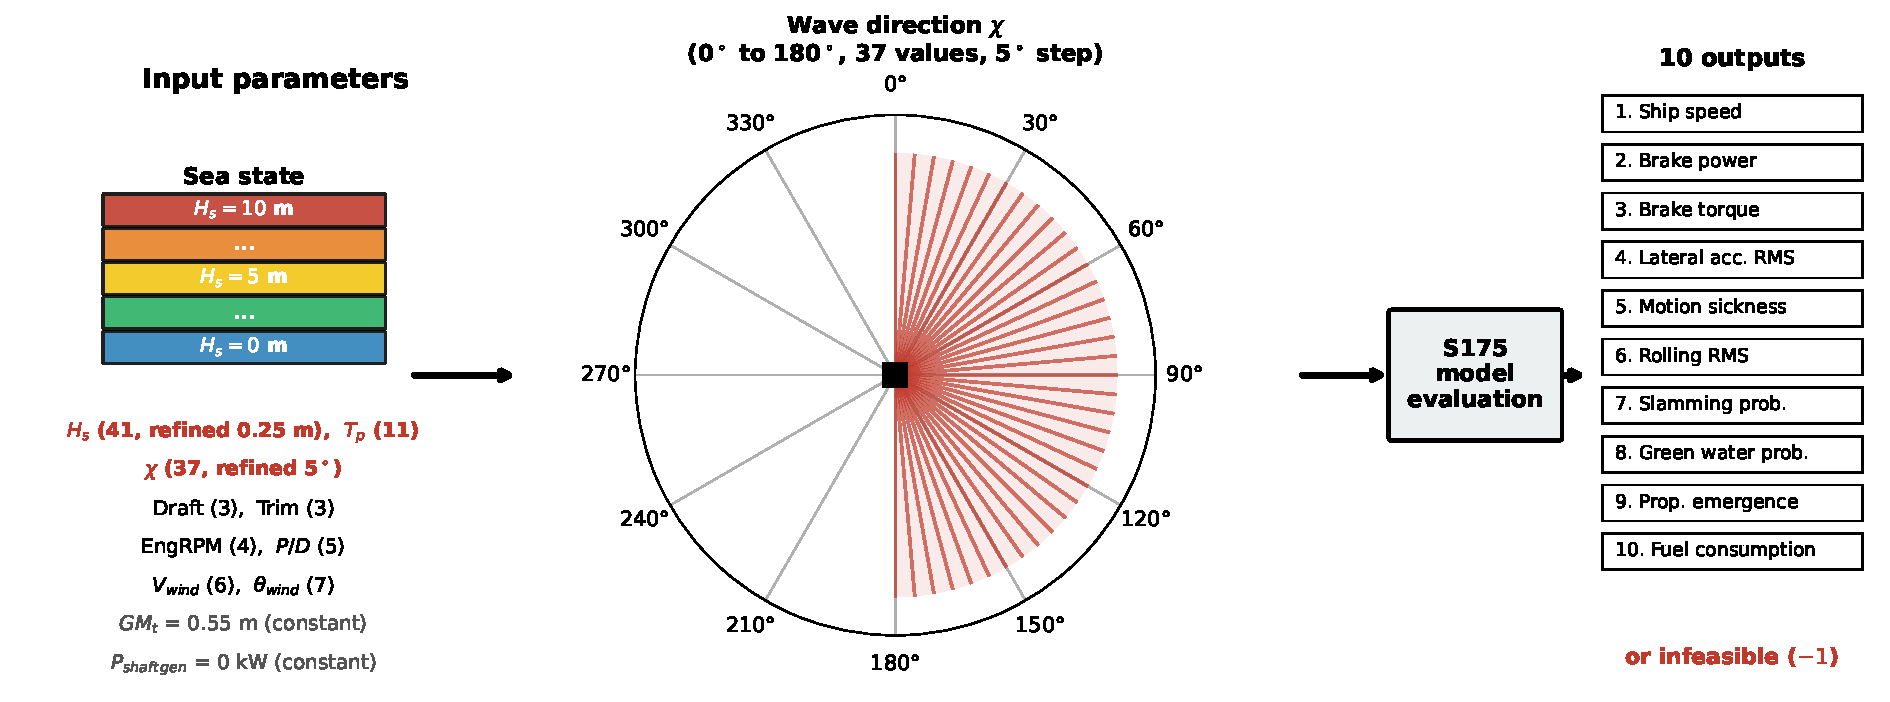
\includegraphics[width=\textwidth]{s175_Dataset-Gen.pdf}
\caption{Dataset generation for the S175 surrogate.}
\label{fig:dataset}
\end{figure*}

The model takes eleven input parameters: mean draft, trim, transverse metacentric height ($GM_t$), engine speed, propeller pitch-to-diameter ratio ($P/D$), shaft generator power, significant wave height ($H_s$), wave peak period ($T_p$), wave direction ($\chi$), relative wind speed, and relative wind direction. For each input combination it returns ten outputs: ship speed, brake power, brake torque, six seakeeping-related indices (lateral acceleration RMS, motion sickness incidence, rolling amplitude RMS, slamming probability, green water probability, and propeller emergence probability), and fuel consumption. The inputs are summarised in \autoref{tab:inputs} and the outputs in \autoref{tab:outputs}; the motion sickness incidence and the three event probabilities are reported by the model, and used throughout this paper, in percent.

\begin{table}[ht]
\centering
\caption{Input parameters of the S175 ship performance model.}
\label{tab:inputs}
\footnotesize
\setlength{\tabcolsep}{10pt}
\renewcommand{\arraystretch}{1.1}
\begin{tabular}{llc}
\toprule
Parameter & Description & Unit \\
\midrule
Draft & Mean draft & \unit{m} \\
Trim & Trim & \unit{m} \\
$GM_t$ & Transverse metacentric height & \unit{m} \\
EngRPM & Engine speed & \unit{rpm} \\
$P/D$ & Propeller pitch-to-diameter ratio & --- \\
$P_{\mathrm{shaft\,gen}}$ & Shaft-generator power & \unit{kW} \\
$H_s$ & Significant wave height & \unit{m} \\
$T_p$ & Wave peak period & \unit{s} \\
$\chi$ & Wave direction & \unit{rad} \\
$V_{\mathrm{wind}}$ & Relative wind speed & \unit{m/s} \\
$\theta_{\mathrm{wind}}$ & Relative wind direction & \unit{rad} \\
\bottomrule
\end{tabular}
\end{table}
% ==============================================================================
% TABLE 2: Output Parameters
% ==============================================================================
\begin{table}[ht]
\centering
\caption{Output parameters of the S175 ship performance model.}
\label{tab:outputs}
\footnotesize
\setlength{\tabcolsep}{12pt}
\renewcommand{\arraystretch}{1.1}
\begin{tabular}{r lc}
\toprule
\# & Output & Unit \\
\midrule
 1 & Ship speed                      & \unit{kn} \\
 2 & Brake power                     & \unit{kW} \\
 3 & Brake torque                    & \unit{kNm} \\
 4 & Lateral acceleration RMS        & $g$ \\
 5 & Motion sickness incidence       & \% \\
 6 & Rolling amplitude RMS           & \unit{\degree} \\
 7 & Slamming probability            & \% \\
 8 & Green water probability         & \% \\
 9 & Propeller emergence probability & \% \\
10 & Fuel consumption                & \unit{kg/nm} \\
\bottomrule
\end{tabular}
\end{table}

Each input parameter was assigned a fixed set of discrete values, and the model was run once for every possible combination of these values. The values used for each input are listed in \autoref{tab:ranges}, where wave and wind directions are given in degrees for readability, although the model itself takes them in radians. Two parameters were held constant: the transverse metacentric height was fixed at $GM_t = 0.55$~m, and the analysis reported here is restricted to the shaft-generator-off condition, $P_\mathrm{shaft\,gen} = 0$~kW. The remaining nine parameters were varied, so that the surrogate maps nine inputs to ten outputs.

\begin{table}[ht] \footnotesize
\centering
\caption{Values of the input parameters in the full factorial design.}
\label{tab:ranges}
\begin{tabular}{lllc}
\hline
Parameter & Range / values & Step & No. of values \\
\hline
Draft (m) & 8.0 to 9.0 & 0.5 & 3 \\
Trim (m) & $-0.75$, 0.00, 0.25 & --- & 3 \\
EngRPM (rpm) & 122.4 to 144.0 & 7.2 & 4 \\
$P/D$ & 0.7 to 1.1 & 0.1 & 5 \\
$H_s$ (m) & 0 to 10 & 0.25 & 41 \\
$T_p$ (s) & \makecell[l]{4.49, 5.19, 5.99, 6.35,\\ 7.33, 8.20, 8.98, 10.37,\\ 12.70, 14.67, 18.50} & --- & 11 \\
$\chi$ (deg) & 0 to 180 & 5 & 37 \\
$V_\mathrm{wind}$ (m/s) & 0 to 25 & 5 & 6 \\
$\theta_\mathrm{wind}$ (deg) & 0 to 180 & 30 & 7 \\
\hline
\end{tabular}
\end{table}

The full factorial combination of these values yields:
\begin{equation}
3 \times 3 \times 4 \times 5 \times 41 \times 11 \times 37 \times 6 \times 7 = 126{,}153{,}720
\label{eq:total}
\end{equation}
cases for the shaft-generator-off condition. Of these cases, 84{,}771{,}762 (67.1972\%) are fully valid, 18{,}581{,}939 (14.7296\%) are fuel-only infeasible, and 22{,}800{,}019 (18.0732\%) are completely infeasible. The model was originally sampled at a low resolution, with the significant wave height in steps of $1.0$~m (eleven values from 0 to 10~m) and the wave direction in steps of $20^\circ$ (ten values from $0^\circ$ to $180^\circ$). At this resolution only a limited number of sea-state conditions are represented, and the wide spacing between sampled points leaves large regions of the input space in which the strongly nonlinear dependence of the outputs on the sea state is poorly captured. To cover a larger number of operating conditions and to produce a denser and more informative dataset for training the surrogate, the sampling was refined in two sea-state parameters, the significant wave height and the wave direction. The significant wave height step was reduced from $1.0$~m to $0.25$~m, increasing the number of wave heights from eleven to forty-one, and the wave direction step was reduced from $20^\circ$ to $5^\circ$, increasing the number of directions from ten to thirty-seven. This refinement narrows the spacing between sampled points and substantially increases the number of cases, so that the surrogate is trained on a finer and more comprehensive coverage of the input space. 
\section{Methodology}\label{sec:method}
This section presents the methodology used to construct the surrogate for the S175 WeatherRouting performance simulator. Constructing this surrogate requires both accurate prediction of the simulator outputs and preservation of its feasibility structure. For feasible operating conditions, the surrogate must predict the ten performance and seakeeping outputs, whereas for infeasible conditions, it must identify which outputs are undefined rather than return apparently valid numerical values. Accordingly, the proposed framework adopts a two-stage architecture in which feasibility classifiers first determine the validity of each operating condition, after which a multi-output regressor predicts the physically defined quantities. The following subsections describe the candidate learning algorithms, the two-stage architecture, the masked-loss formulation used for fuel-only infeasible cases, the safety-aware asymmetric loss, and the model-training procedure. The complete workflow for constructing the two-stage surrogate is summarised in~\autoref{alg:surrogate}.

\begin{algorithm}[ht!]
\scriptsize
\caption{Construction of the two-stage S175 surrogate}
\label{alg:surrogate}
\begin{algorithmic}[1]
\Require Dataset $\mathcal{D}=\{(\mathbf{x}_i,\mathbf{y}_i)\}$, where infeasible outputs are encoded as $-1$
\Require Candidate weight pairs $A=\{1.0,1.5,2.0,3.0,5.0\}\times\{1.5,1.0,0.8,0.67,0.5,0.33\}$ for $(\alpha_{\mathrm{speed}},\alpha_{\mathrm{other}})$
\State Draw a 5\% screening subsample (6{,}306{,}419 cases) from $\mathcal{D}$, stratified by feasibility category, significant-wave-height band, wave direction, and wind speed
\State Divide the screening subsample into screening-training, screening-validation, and held-out selection partitions
\State Compare Random Forest, XGBoost, and MLP models, each as a single $-1$-target regressor and as a classifier with a valid-row regressor, on a separate 80/10/10 partition of the subsample over three seeds, and select the MLP family
\Statex \textbf{Screening-stage loss selection (joint weight grid)}
\State Form the screening regression set from fully valid and fuel-only-infeasible screening cases, with the fuel-consumption mask
\For{each pair $(\alpha_s,\alpha_o)\in A$ and each of five random seeds}
\State Train the ten-output screening regressor (final regressor architecture) with the masked loss, $\alpha_j\gets\alpha_s$ for ship speed and $\alpha_j\gets\alpha_o$ for the other nine outputs, with early stopping on the screening-validation partition
\State Record, on the held-out selection partition, each output's conservative-direction rate on rows with a strictly positive target value, the standardised MAE, and $R^2$
\EndFor
\State Apply the prespecified selection rule: a pair is eligible only if all ten outputs err preferentially on their conservative side in every seed
\If{no pair is eligible}
\State Extend the candidate set with $\alpha_{\mathrm{other}}\in\{0.25,0.20\}$ and repeat the joint-grid training and evaluation \Comment{not activated}
\EndIf
\State Among eligible pairs, select the pair with the lowest mean standardised MAE, breaking exact ties by the higher mean $R^2$
\State Only $(\alpha_{\mathrm{speed}},\alpha_{\mathrm{other}})=(1.5,0.33)$ is eligible; select it
\Statex \textbf{Independent final training campaign}
\State Label every case as \emph{fully valid}, \emph{fuel-only infeasible}, or \emph{completely infeasible}
\State Independently split $\mathcal{D}$ into training, validation, and test subsets in proportions of 80/10/10, stratified by feasibility category, significant-wave-height band, and wind-speed band
\State Standardise inputs and regression targets using statistics computed from the final training subset only
\State Train classifier $C_1$ on all final-training cases to detect complete infeasibility
\State Train classifier $C_2$ on final-training cases that are not completely infeasible to detect fuel-only infeasibility
\State Select thresholds $\tau_1$ and $\tau_2$ on the final validation subset as the highest thresholds maintaining infeasible-class recall $\geq0.99$
\State Form the regression set from fully valid and fuel-only infeasible final-training cases
\State Train regressor $R$ using the masked asymmetric loss with $\alpha_{\mathrm{speed}}=1.5$ and $\alpha_j=0.33$ for the other nine outputs
\State Define the primary test subset by excluding every final-test row appearing anywhere in the screening subsample
\State \Return classifiers $C_1$ and $C_2$ with thresholds $\tau_1$ and $\tau_2$, and regressor $R$
\Statex \textbf{Inference for a new input $\mathbf{x}$}
\State \textbf{if} $C_1(\mathbf{x})>\tau_1$ \textbf{then} return all outputs $=-1$
\State \textbf{else} predict outputs using $R(\mathbf{x})$; \textbf{if} $C_2(\mathbf{x})>\tau_2$ \textbf{then} set fuel consumption $=-1$
\end{algorithmic}
\vspace{-3pt}

\end{algorithm}

The overall methodology followed in this work is summarised in \autoref{fig:methodology}. The dataset is first generated by evaluating the S175 model over the refined full factorial design and is then split, in a stratified manner, into training, validation, and test subsets. Three families of learning algorithms, namely Random Forest, Extreme Gradient Boosting, and a multi-layer perceptron, are compared in a preliminary screening on a stratified subsample under identical conditions, and the multi-layer perceptron is selected on the basis of these results and its ability to predict all outputs jointly. The surrogate is then constructed as a two-stage model: a feasibility classification stage that reproduces the two infeasibility modes of the simulator, and a regression stage that predicts the ten outputs. The two asymmetric-loss weights are selected in the screening campaign over a joint grid of candidate pairs, every pair trained under the final surrogate's masked-loss protocol and judged by a selection rule fixed before the grid was run, after which the final regressor is trained once on the fully valid and fuel-only-infeasible final-training cases using the masked, per-output asymmetric loss. The resulting two-stage surrogate is finally validated on the held-out test set, under structured holdout regimes that withhold entire input levels, operating regions, and envelope corners from training, and against the original model at input combinations lying between the grid points. The following subsections describe each of these components in detail.

\begin{figure*}[ht!]
\centering
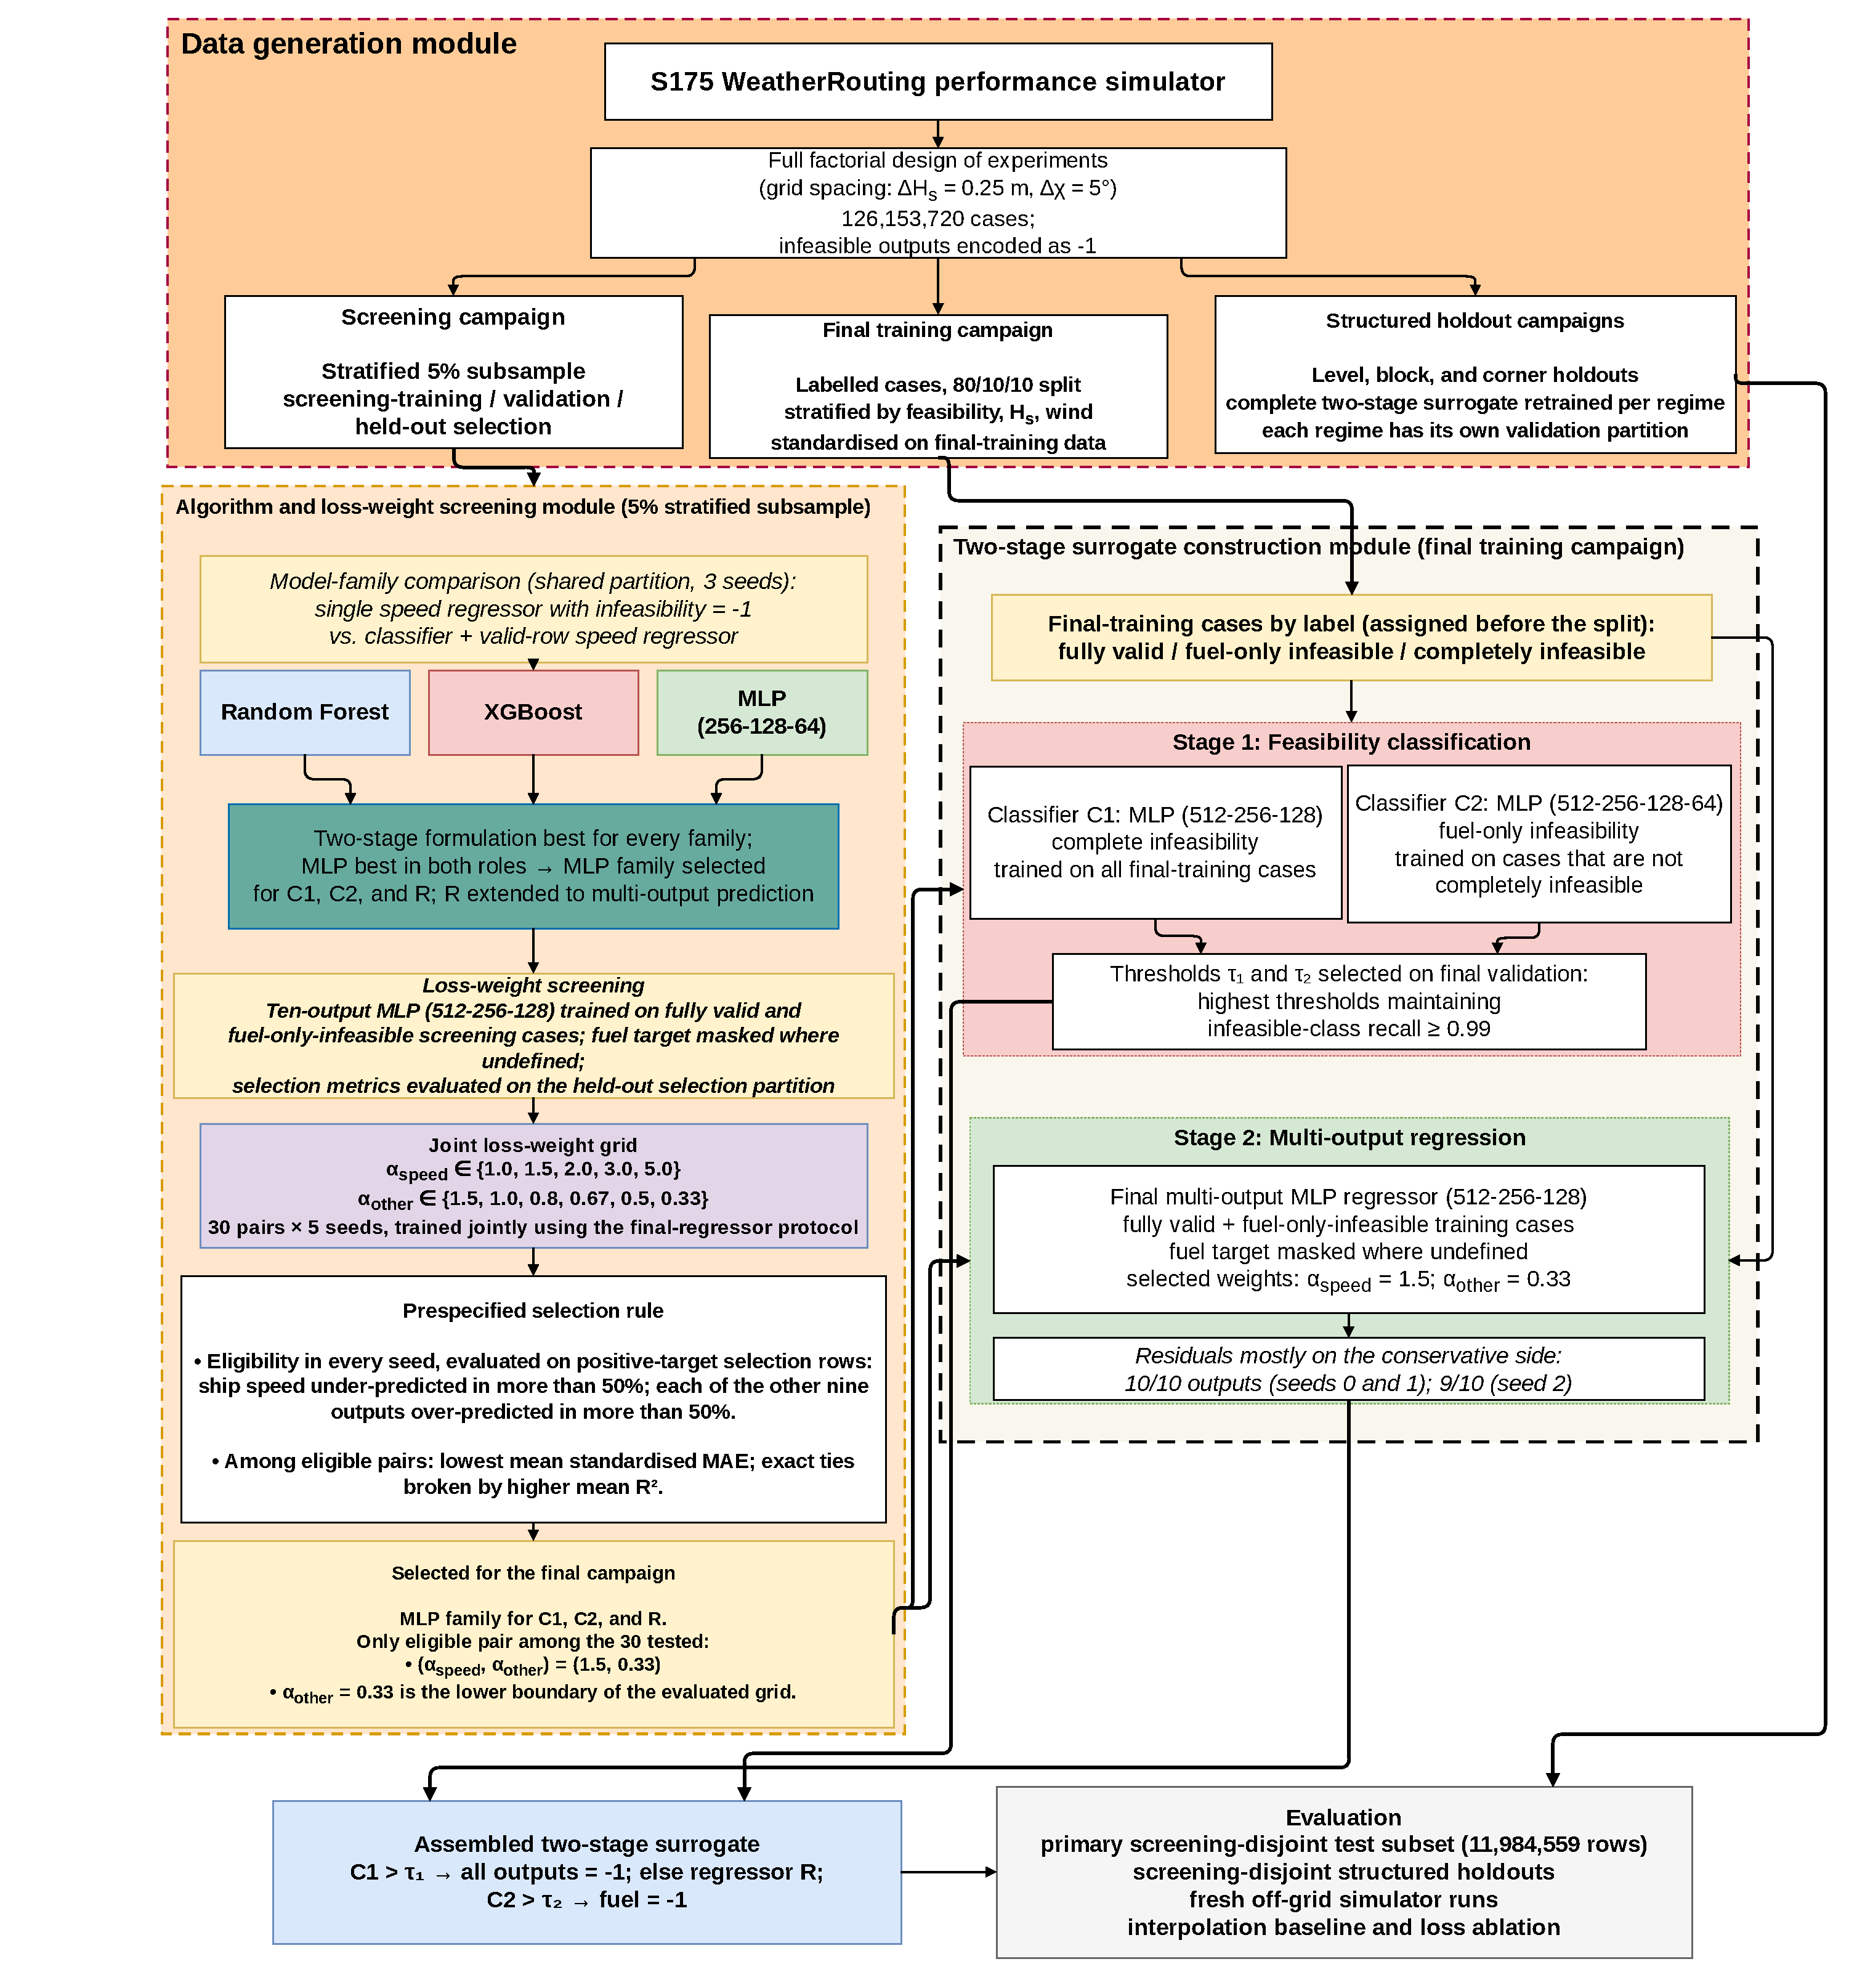
\includegraphics[width=0.85\textwidth]{S175ML-V5-F.drawio-updated-28-09-2026.drawio.pdf}
\caption{Methodology for constructing and evaluating the two-stage S175 surrogate}
\label{fig:methodology}
\end{figure*}
\subsection{Candidate learning algorithms}

Three supervised-learning families were evaluated as candidate surrogate models: Random Forests, gradient-boosted decision trees implemented through eXtreme Gradient Boosting (XGBoost), and multi-layer perceptrons (MLPs). These families represent complementary learning strategies based on bagging, sequentially boosted trees, and neural-network function approximation, respectively. Random Forests have been applied as surrogates in simulation-based engineering optimisation~\cite{jiao2025rf}, while XGBoost and neural networks have demonstrated strong performance in approximating nonlinear simulation responses~\cite{stevanovic2024}. MLP-based surrogates have also been used to approximate high-fidelity engineering simulations and ship-hydrodynamic quantities~\cite{ablanque2025,matai2025,rechevilanova2024}.

The three model families were screened using the same stratified data subset, input and output definitions, data split, and evaluation metrics, thereby enabling a consistent comparison of their predictive performance. The screening used ship speed as the regression target and complete infeasibility as the classification target, and it did not reproduce the final ten-output configuration (\autoref{sec:selection}, \autoref{tab:algselect}). An important consideration was that the S175 simulator produces ten outputs from the same operating condition, with several outputs linked through the underlying propulsion, resistance, and seakeeping relationships. A joint multi-output model can therefore learn these responses simultaneously rather than treating each output as an independent prediction problem. Although multi-output implementations of Random Forests and gradient boosting are available, an MLP provides a direct mechanism for learning a shared nonlinear representation through its hidden layers and producing all ten predictions through a single output layer. Based on the screening results and this architectural suitability, the MLP was selected for both the feasibility-classification and the regression stages, while the tree-based methods were retained as screening baselines.


\subsection{Two-stage architecture}

The surrogate architecture was designed to reproduce the output-validity structure of the S175 simulator. For a given operating condition, the simulator may return all ten outputs, return nine valid outputs with only fuel consumption undefined, or return no valid output. A conventional regression model would not explicitly distinguish among these outcomes. Separating feasibility identification from continuous-response prediction is consistent with recent surrogate-modelling frameworks that represent simulation convergence or design validity as a classification problem and restrict continuous-output prediction to configurations classified as feasible~\cite{durkin2024feasibility,aghayev2025classification,mahajan2025feasibility}. The proposed architecture therefore uses two feasibility classifiers to identify complete and fuel-only infeasibility, followed by a conditional multi-output regressor that predicts only the outputs defined for the queried condition. This arrangement suppresses numerical predictions for conditions classified as infeasible and reproduces the simulator's feasibility behaviour to the accuracy quantified in~\autoref{sec:results}.

Complete infeasibility occurs when the simulator cannot compute a ship speed for the prescribed engine RPM, propeller setting, and operating conditions; consequently, none of the ten outputs is defined. Fuel-only infeasibility occurs when the speed, propulsion, and seakeeping calculations remain valid, but the converged brake power and the prescribed engine speed lie outside the admissible region of the engine's SFC map (\autoref{sec:model}), preventing the calculation of a valid fuel-consumption value. Completely infeasible inputs are therefore excluded from regression, whereas fuel-only infeasible inputs retain predictions for the nine valid outputs and suppress only the fuel-consumption prediction.


\subsection{Masked loss for fuel-only infeasible cases}

The classification stage determines which simulator outputs are valid for each input, but this output-dependent validity must also be incorporated into regression training. In particular, fuel-only infeasible cases provide valid targets for nine outputs while the fuel-consumption target remains undefined. Recent surrogate-modelling work treats outputs from unsuccessful simulator evaluations as unavailable for regression to prevent them from distorting the learned response~\cite{durkin2024feasibility}. Similarly, multi-task learning models with incomplete output labels use masked losses to exclude unavailable targets from backpropagation while retaining the available targets from the same samples~\cite{peteani2024masked}.

Accordingly, removing fuel-only infeasible samples entirely would discard valid supervision for the other nine outputs, whereas replacing the undefined fuel-consumption value with an artificial numerical target would introduce non-physical supervision. A binary validity mask is therefore assigned to each sample--output pair during loss calculation. For fuel-only infeasible samples, the mask sets the fuel-consumption contribution to zero while retaining the loss contributions of the other nine outputs. The resulting loss is normalised by the number of valid target elements, as formalised in \autoref{eq:masked}. Consequently, fully feasible samples contribute to the training of all ten outputs, fuel-only infeasible samples contribute to the nine defined outputs, and completely infeasible samples are excluded from regression training.
\subsection{Asymmetric least-squares loss}

The masked loss described above determines which valid targets contribute to regression training, whereas the present component determines how errors in those targets are penalised. For route evaluation, the direction of a prediction error can be operationally important in addition to its magnitude because over-prediction and under-prediction do not necessarily have equivalent consequences. This is consistent with the forecasting principle that the loss function should reflect the decision context in which the predictions will be used~\cite{gneiting2011,elliott2005}. Recent engineering research has similarly used direction-dependent loss functions to bias neural-network predictions toward domain-defined conservative estimates~\cite{habib2026asymmetric}. This consideration is relevant to weather-routing optimisation, which evaluates trade-offs among attainable speed or voyage duration, propulsion and fuel demand, and seakeeping-related safety constraints~\cite{pennino2020,kytariolou2022,han2025weather}.

The conservative direction assigned to each output is an application-specific design choice based on how that quantity enters route evaluation, rather than a convention established in previous ship-surrogate studies. This choice is consistent with weather-routing formulations that evaluate whether a commanded speed is attainable, reject operating points outside the engine operating envelope, minimise fuel consumption, and impose upper limits on seakeeping responses~\cite{pennino2020,kytariolou2022}. Accordingly, ship speed is preferably under-predicted so that the surrogate does not overstate the speed attainable under the specified operating and environmental conditions. Brake power, brake torque, and fuel consumption are preferably over-predicted to avoid understating propulsion loading and fuel demand. The six seakeeping outputs are also preferably over-predicted because, as defined in~\autoref{sec:model}, they comprise response magnitudes, incidence, and event probabilities for which larger values indicate a more severe vessel response or a higher likelihood of an adverse event. The resulting directional bias is distributional and does not provide a pointwise safety guarantee. A symmetric loss such as the mean squared error assigns identical penalties to positive and negative errors of equal magnitude and therefore cannot encode this output-dependent preference~\cite{newey1987}.


To encode the preferred direction, an output-specific asymmetric squared-error loss is used. Following the asymmetric least-squares principle, positive and negative residuals are assigned different weights~\cite{newey1987}. For sample $i$ and output $j$, let $e_{ij}=\hat{y}_{ij}-y_{ij}$. The corresponding loss is
\begin{equation}
\ell_{ij}=
\begin{cases}
\alpha_j e_{ij}^{2}, & e_{ij}>0,\\
e_{ij}^{2}, & e_{ij}\leq0,
\end{cases}
\label{eq:asym}
\end{equation}
and, with the binary validity mask $m_{ij}$ of the preceding subsection, the loss of a mini-batch is
\begin{equation}
L=\frac{\sum_{i,j} m_{ij}\,\ell_{ij}}{\sum_{i,j} m_{ij}},
\label{eq:masked}
\end{equation}
where both sums run over all samples and outputs of the mini-batch and $e_{ij}$ is computed on the standardised targets. In \autoref{eq:asym}, $\alpha_j>1$ penalises over-prediction more heavily and therefore biases output $j$ toward under-prediction, whereas $\alpha_j<1$ penalises under-prediction more heavily relative to over-prediction and therefore biases the output toward over-prediction. Ship speed is assigned the separate weight $\alpha_{\mathrm{speed}}$, while the remaining nine outputs share the weight $\alpha_{\mathrm{other}}$. Because all ten outputs are predicted through shared hidden layers, changing either weight can affect every output; the two weights were therefore selected jointly rather than through successive independent sweeps. The candidate set comprised $\alpha_{\mathrm{speed}}\in\{1.0,1.5,2.0,3.0,5.0\}$ and $\alpha_{\mathrm{other}}\in\{1.5,1.0,0.8,0.67,0.5,0.33\}$, giving thirty pairs. The uniform settings arise as points of this grid: $(1.0,1.0)$ recovers the symmetric mean squared error, and $(1.5,1.5)$ is the uniform asymmetric weighting revisited in the loss-configuration ablation of \autoref{sec:selection}. Each pair was trained from five random seeds on the stratified 5\% screening subsample using the same architecture, masked loss, optimisation settings, batch size of 65{,}536, and automatic mixed-precision training as the final regressor. Repeating each configuration across multiple seeds was used to quantify variability across stochastic training runs~\cite{bouthillier2021variance}. The screening subsample was partitioned into training, validation, and selection subsets in proportions of 80\%, 10\%, and 10\%, respectively. Training was performed on the screening-training partition, early stopping was based on the screening-validation partition, and weight selection used only the held-out selection partition. Every row in the screening subsample was subsequently excluded from the primary test subset, thereby separating loss-weight selection from final performance evaluation and reducing selection bias~\cite{cawley2010selection}.
The selection rule was specified before the results of the joint-grid campaign were examined. Directional rates were computed on selection rows with strictly positive target values. A pair was eligible only if ship speed was under-predicted in more than half of these rows and each of the remaining nine outputs was over-predicted in more than half, in every one of the five seeds. Among eligible pairs, the pair with the lowest mean standardised MAE was to be selected, with mean $R^2$ used only to break an exact tie. Each output's MAE was normalised by that output's standard deviation on the selection partition before averaging across outputs and seeds. The asymmetric weighting is applied together with the validity mask introduced in the preceding subsection, so that the fuel-consumption error is direction-weighted when a valid fuel target exists and omitted when fuel consumption is infeasible. The joint-grid results, the selected configuration, and the boundary of the evaluated weight grid are reported in \autoref{tab:alphagrid} and \autoref{fig:alphagrid}.


\subsection{Training procedure}
The dataset was divided into training, validation, and test subsets in proportions of 80\%, 10\%, and 10\%, respectively. The split was stratified by feasibility class, significant-wave-height band ($H_s\leq2$, $2<H_s\leq5$, $5<H_s\leq8$, and $H_s>8$~m), and wind-speed band ($V_{\mathrm{wind}}\in\{0,5\}$, $\{10,15\}$, or $\{20,25\}$~m/s), so that the proportions of fully valid, fuel-only infeasible, and completely infeasible cases were preserved across the three subsets. Because each row of the full-factorial database corresponds to a unique input combination, the random row-level split primarily evaluates interpolation within the densely sampled factorial lattice rather than generalisation to systematically withheld regions of the input space~\cite{wang2024extrapolation}. To assess generalisation beyond this random interpolation setting, the structured level, block, and corner holdouts described below were evaluated separately. The input parameters were standardised to zero mean and unit variance using statistics computed exclusively from the training subset, which improves the conditioning of neural-network optimisation~\cite{lecun1998}. The ten regression targets were also standardised using means and standard deviations computed on the training rows that are not completely infeasible, excluding the $-1$ infeasibility codes, so that the fuel-consumption statistics are computed from fully valid rows only, and so that outputs with larger numerical scales, such as brake power, did not dominate the multi-output loss. Predictions were transformed back to physical units and clamped to the physically admissible range of each output before evaluation. The bounds were physical rather than data-derived: non-negativity for ship speed, brake power, brake torque, lateral-acceleration RMS, roll RMS, and fuel consumption, and the interval $[0,100]$ for the four probability and percentage outputs. Clamping affected an appreciable fraction of predictions only for the probability outputs, whose true values concentrate at zero, by clipping slightly negative predictions to zero. This occurred for up to 28.7\% of the green-water-probability predictions on the random split and at most 16.1\% in the corner regime. Its effect on $R^2$ was negligible, with the largest change in any per-output $R^2$ remaining below $2.3\times10^{-5}$ on both the random split and the corner regime, whereas on the random split it reduced the MAE by 13.1\% for propeller emergence probability, 9.1\% for green water probability, 8.6\% for motion sickness incidence, and 4.0\% for slamming probability; all reported MAE values refer to clamped predictions. For masked fuel targets, the arbitrary infeasible encoding was replaced by the training mean of the valid fuel-consumption values, which maps to zero in standardised space and contributes no gradient through the mask.

The regression network is a multi-layer perceptron with three hidden layers containing 512, 256, and 128 units. Each hidden layer comprises a linear transformation followed by batch normalisation~\cite{ioffe2015batchnorm} and a ReLU activation, and the network uses a linear output head for the ten targets. Both feasibility classifiers use the same three hidden layers as the regressor and a single-logit output head, and the fuel-only classifier adds a fourth hidden layer of 64 units. The classifiers were trained with the binary cross-entropy loss computed on the logit, without class weighting or resampling, and their decision thresholds are applied to the sigmoid output, a case being classified as infeasible when this output exceeds the threshold. The hidden-layer sizes were adopted from a preliminary configuration search on the 5\% screening subsample, in which regressor and classifier candidates including 256--128--64, 512--256--128, and 512--256--128--64 hidden units were compared in single training runs using the mean of the ten per-output MAEs in physical units for regressors and the F1 score for classifiers on the held-out partition of a separate 80/10/10 split of the subsample; no rows of the primary test subset were used in that search. The fuel-only classifier was trained only on cases that were not completely infeasible, corresponding to the population for which fuel feasibility is assessed during inference. All networks were trained with the Adam optimiser~\cite{kingma2015}, a learning rate of $10^{-3}$, a batch size of 65{,}536 selected through a throughput pilot, CUDA automatic mixed-precision training with FP16 autocasting and dynamic gradient scaling~\cite{micikevicius2018mixedprecision}, a maximum of 200 epochs, and early stopping with a patience of 15 epochs. The regression network minimised the masked asymmetric loss defined in the preceding subsections. The validation subset was used for early stopping: training was halted when the validation loss ceased to improve, thereby limiting overfitting and retaining the model state with the best validation performance~\cite{prechelt1998}. The decision thresholds of the two feasibility classifiers were also selected on the validation subset rather than fixed at the conventional value of 0.5. The deployment-critical error was defined as a false negative for the infeasible class, in which the surrogate returns numerical outputs for a condition that the simulator identifies as infeasible. Accordingly, each threshold was searched from 0.01 to 0.99 in steps of 0.01 and set to the largest value for which validation recall of the infeasible class remained at least 0.99. This selects the highest threshold, and hence the fewest false alarms, that still satisfies the prespecified recall constraint. The held-out test subset was used only for the final evaluation reported in \autoref{sec:results}.

Beyond the random split, structured holdout regimes were constructed to evaluate generalisation to systematically withheld operating conditions. In the level-holdout regimes, complete values of individual inputs were withheld from training and used for testing: $H_s\in\{0.25,5.00,9.75\}$~m, $\chi\in\{5^\circ,90^\circ,175^\circ\}$, draft $=8.5$~m, and $V_{\mathrm{wind}}\in\{5,20\}$~m/s. In the block-holdout regime, the joint region of the thirteen wave heights $H_s\in\{7.00,7.25,\dots,10.00\}$~m and the eleven wave directions $\chi\in\{65^\circ,70^\circ,\dots,115^\circ\}$ was withheld. In the corner regime, every row with $H_s\geq8.75$~m or $V_{\mathrm{wind}}=25$~m/s was withheld, so each test condition lay beyond the retained training range in at least one of these two variables. In every regime, the retained rows were repartitioned into training and validation subsets stratified by feasibility class, significant-wave-height band, and wind-speed band. The model family, the network architecture, and the loss weights were selected once on the screening subsample, which was drawn from the complete factorial domain. Although the screening rows are removed from every holdout test set, the structured holdouts evaluate the transfer of the surrogate trained with these globally selected settings rather than a fully nested selection repeated within each regime~\cite{cawley2010selection}.
\subsection{Implementation and experimental settings}\label{sec:env}
The surrogate pipeline was implemented in Python 3.14.4 using PyTorch 2.13.0 with CUDA 13.0 for the training and inference of the surrogate networks and NumPy 2.5.1 for data handling; the model-family screening used the scikit-learn MLP and Random Forest and the XGBoost library implementations with the hyperparameters given in \autoref{sec:selection}. All training and evaluation ran on a single workstation equipped with an Intel Xeon E5-4620~v2 CPU at 2.60~GHz and an NVIDIA Quadro RTX~5000 GPU with 16~GB of memory, the same workstation used for the computational comparison of \autoref{sec:speed}, with all networks trained entirely on the GPU under the mixed-precision configuration of the preceding subsection. Under these settings, training the reference-seed models on the full dataset required approximately 38 minutes for the regressor, 84 minutes for the complete-infeasibility classifier, and 43 minutes for the fuel-only classifier, so one complete seed of the two-stage surrogate trains in under three hours, and the 150 screening-stage trainings of the loss-weight grid completed in approximately seven hours in total. 
\section{Results}\label{sec:results}
This section reports the performance of the surrogate trained with the configuration selected in \autoref{sec:method}. Unless stated otherwise, the reported results use the screening-disjoint test subset of the random split. The original held-out test subset contains 12{,}615{,}370 rows. Removing the 630{,}811 rows, corresponding to 5.00\%, that also occur in the earlier screening subsample leaves 11{,}984{,}559 rows that were not used during model-family screening, loss-weight selection, final training, validation, or threshold calibration. This screening-disjoint subset therefore serves as the primary test set of the paper. The same exclusion is applied to every structured-holdout test set. Evaluating the complete test subset instead changes none of the reported $R^2$ values or over-prediction rates at the displayed precision and alters three MAE values only in their last displayed digit. On the random split, all three networks were trained with random seeds 0, 1, and 2; each structured holdout regime was trained with seed 0. Unless stated otherwise, the detailed tables and figures report the run with seed 0, which was the first run trained and is the default of the training script, while the three-seed mean, standard deviation, and minimum result for each regression output are reported with the regression results in \autoref{sec:regacc}. Seed 0 is not the best run on every output: it attains the highest $R^2$ for six and the lowest MAE for six of the ten outputs.

\subsection{Model and loss selection}\label{sec:selection}

This subsection reports the preliminary model-family screening, the joint selection of the asymmetric-loss weights, and the subsequent loss-configuration ablation.

The candidate model families were compared on one 80/10/10 partition of the stratified 5\% screening subsample into training, validation, and selection partitions, separate from the partition used for the loss-weight grid and stratified by significant-wave-height band, wind-speed band, and complete-infeasibility status. For each family, two formulations were trained from three random seeds (\autoref{tab:algselect}). In the single-regressor formulation, one ship-speed regressor was trained on all rows with complete infeasibility encoded as a target value of $-1$, and a row was classified as infeasible when its prediction did not exceed a threshold. In the two-stage formulation, a binary classifier of complete infeasibility was followed by a ship-speed regressor trained on valid rows only. In both formulations, the detection threshold was the point of maximum F1 on the validation partition, unlike the recall-constrained thresholds of the final classifiers, and the speed MAE and $R^2$ were computed on all 516{,}684 selection rows with a valid speed, so that both formulations were scored on identical rows. The Random Forest used 100 trees, a maximum depth of 20, and a minimum leaf size of 5. XGBoost used 200 histogram-based trees, a maximum depth of 8, a learning rate of 0.1, a minimum child weight of 5, and row and column subsampling rates of 0.8. The screening MLP (scikit-learn) contained three hidden layers of 256, 128, and 64 units and was trained using ReLU activations, the Adam optimiser with an adaptive learning rate starting at $10^{-3}$, a batch size of 1{,}024, at most 300 iterations, and early stopping on 10\% of its training rows.

\begin{table*}[ht]
\footnotesize
\centering
\caption{Model-family screening on the 5\% subsample (mean $\pm$ SD over three seeds).}
\label{tab:algselect}
\begin{tabular}{llcccc}
\hline
Algorithm & Formulation & Infeasibility F1 & Missed infeasible & Speed MAE [kn] & Speed $R^2$ \\
\hline
Random Forest & Single regressor & $0.9831\pm0.0000$ & $3{,}276\pm33$ & $0.191\pm0.000$ & $0.8776\pm0.0001$ \\
 & Two-stage & $0.9872\pm0.0001$ & $1{,}314\pm56$ & $0.048\pm0.000$ & $0.9993\pm0.0000$ \\
XGBoost & Single regressor & $0.9520\pm0.0003$ & $6{,}431\pm180$ & $0.791\pm0.010$ & $0.5290\pm0.0048$ \\
 & Two-stage & $0.9897\pm0.0004$ & $1{,}170\pm105$ & $0.056\pm0.001$ & $0.9992\pm0.0000$ \\
Multi-layer perceptron & Single regressor & $0.9921\pm0.0019$ & $1{,}319\pm422$ & $0.160\pm0.041$ & $0.9282\pm0.0103$ \\
 & Two-stage & $\mathbf{0.9947\pm0.0007}$ & $\mathbf{540\pm108}$ & $\mathbf{0.025\pm0.001}$ & $\mathbf{0.9999\pm0.0000}$ \\
\hline
\end{tabular}
\end{table*}

For every family, the two-stage formulation detected complete infeasibility more reliably and predicted ship speed considerably more accurately than the single regressor, whose speed MAE was approximately four to fourteen times larger. The MLP gave the best result in both roles, with an infeasibility F1 of $0.9947$, 540 missed infeasible cases, and a speed MAE of 0.025~kn in the two-stage formulation, and was therefore carried forward as the model family for both feasibility classification and multi-output regression. The screening addressed ship speed and complete infeasibility only; it therefore motivates the choice of model family and of the two-stage architecture but does not compare the families in the final ten-output configuration.

 The results of the joint-grid experiment conducted according to the selection protocol described in \autoref{sec:method} are presented in \autoref{tab:alphagrid}. Panel~(a) reports the minimum number of outputs satisfying their prescribed conservative direction across the five seeds, while Panel~(b) reports the corresponding mean standardised MAE.
\begin{table}[ht]
\footnotesize
\centering
\caption{Joint evaluation of the asymmetric-loss weights on the screening subsample.}
\label{tab:alphagrid}
\begin{tabular}{cccccc}
\toprule
& \multicolumn{5}{c}{$\alpha_{\mathrm{speed}}$} \\
\cmidrule(lr){2-6}
$\alpha_{\mathrm{other}}$ & 1 & 1.5 & 2 & 3 & 5 \\
\midrule
\multicolumn{6}{l}{\emph{(a) Worst-seed conservative-direction count [of 10]}} \\
1.5 & 1 & 2 & 2 & 1 & 2 \\
1 & 2 & 2 & 1 & 4 & 4 \\
0.8 & 5 & 4 & 4 & 6 & 2 \\
0.67 & 4 & 6 & 6 & 7 & 5 \\
0.5 & 7 & 8 & 7 & 9 & 7 \\
0.33 & 9 & \textbf{10} & 9 & 9 & 9 \\
\midrule
\multicolumn{6}{l}{\emph{(b) Mean standardised MAE over five seeds [\% of SD]}} \\
1.5 & 1.76 & 1.77 & 1.80 & 1.86 & 1.68 \\
1 & 1.84 & 1.75 & 1.78 & 1.82 & 1.79 \\
0.8 & 1.93 & 1.83 & 1.92 & 1.73 & 1.96 \\
0.67 & 1.80 & 1.87 & 1.75 & 1.86 & 2.02 \\
0.5 & 1.90 & 2.02 & 1.84 & 2.08 & 2.02 \\
0.33 & 2.14 & \textbf{2.21} & 2.00 & 1.96 & 2.06 \\
\bottomrule
\end{tabular}
\end{table}

Only $(\alpha_{\mathrm{speed}},\alpha_{\mathrm{other}})=(1.5,0.33)$ satisfied the eligibility requirement for all ten outputs in every seed. The selection was therefore determined by directional compliance alone; neither the standardised-MAE criterion nor the $R^2$ tie-break was exercised. Across the five seeds, the selected configuration produced a mean standardised MAE of $2.21\pm0.12\%$ of the target standard deviation, whereas the mean values across the complete grid ranged from 1.68\% to 2.21\%, so the selected pair has the highest mean standardised MAE of the grid. This quantifies the accuracy trade-off associated with achieving the prescribed conservative direction for every output.

The selected value $\alpha_{\mathrm{other}}=0.33$ is the lower boundary of the evaluated grid. Consequently, the experiment identifies the only eligible pair among the 30 evaluated configurations but does not establish that $0.33$ is optimal among intermediate or smaller untested values. The prespecified extension to $\alpha_{\mathrm{other}}\in\{0.25,0.20\}$ was not activated because an eligible pair had already been identified. A finer investigation of the loss-weight boundary is left for future work. The directional-compliance and accuracy patterns across the complete grid are visualised in \autoref{fig:alphagrid}.

\begin{figure}[ht!]
\centering
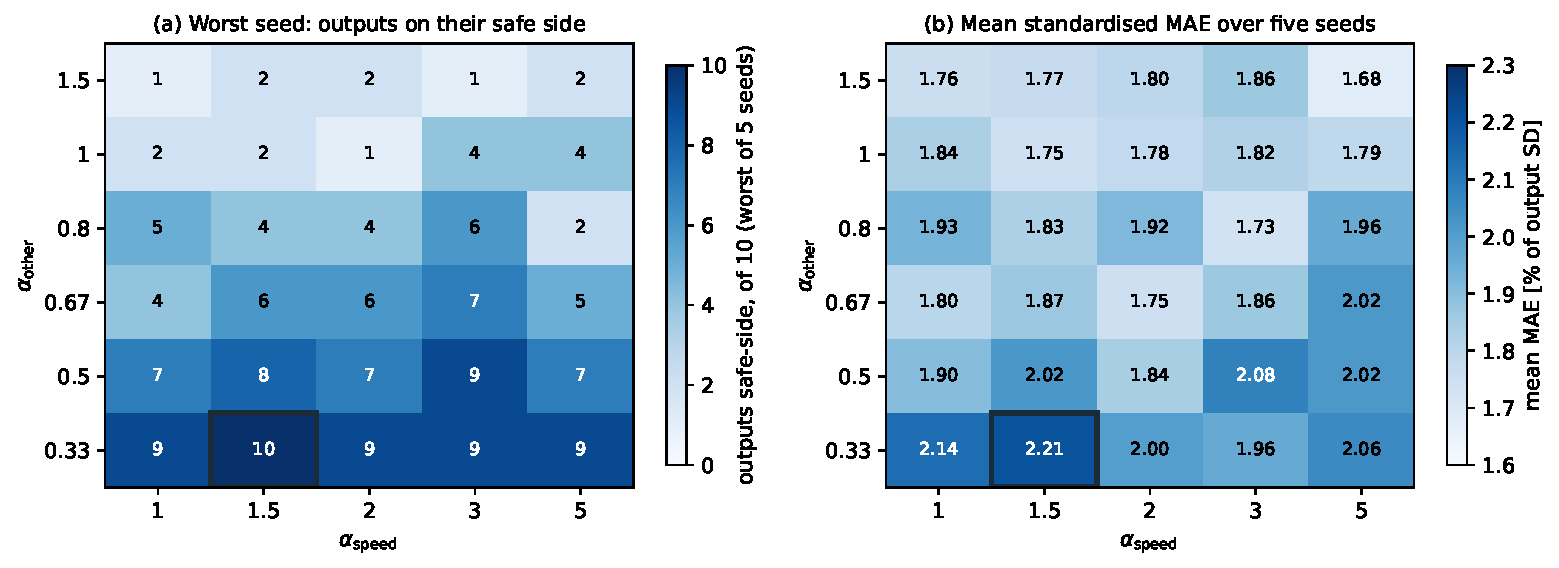
\includegraphics[width=\linewidth]{fig_alpha_grid.pdf}
\caption{Joint asymmetric-loss weight grid: (a) worst-seed conservative-direction count; (b) mean standardised MAE.}
\label{fig:alphagrid}
\end{figure}

The effects of batch-normalisation placement, masked training, and output-specific weighting were examined using five regressors trained under the protocol of \autoref{sec:method} and evaluated on identical screening-disjoint test rows. The first arm reproduces the initial configuration: uniform $\alpha=1.5$ for all ten outputs, no fuel mask, exclusion of fuel-only-infeasible rows from training, and batch normalisation after activation. The second arm retains the unmasked data handling but uses the corrected batch-normalisation placement. The remaining three arms use masked training and differ only in their weighting: uniform $\alpha=1.5$, symmetric $\alpha=1.0$, and the selected output-specific weights. Comparison of the corrected unmasked arm with the uniform masked arm captures the combined effect of masking the undefined fuel target and retaining the fuel-only infeasible cases during regression training. The initial and corrected unmasked arms place three and two outputs on their specified conservative sides, respectively, while the uniform and symmetric masked arms place one and six outputs on their conservative sides. Only the selected output-specific masked configuration places all ten outputs preferentially on their prescribed conservative error sides. \autoref{tab:lossablation} lists the over-prediction rates, and \autoref{fig:lossablation} visualises the error-direction results for the five configurations.

\begin{figure*}[ht!]
\centering
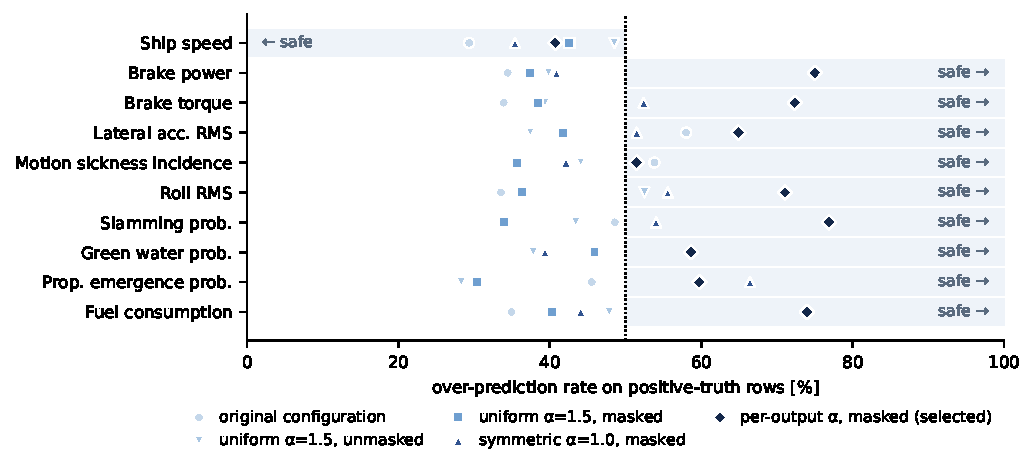
\includegraphics[width=0.9\textwidth]{fig_loss_ablation_safety.pdf}
\caption{Over-prediction rate per output for the five loss configurations.}
\label{fig:lossablation}
\end{figure*}

\begin{table*}[ht]
\centering
\caption{Loss-configuration ablation: over-prediction rate [\%] (\checkmark{} = conservative side).}
\label{tab:lossablation}
\footnotesize
\setlength{\tabcolsep}{3.5pt}
\renewcommand{\arraystretch}{1.1}
\begin{tabular}{llccccc}
\toprule
& &
\makecell{Original\\config.} &
\makecell{Unmasked\\uniform\\($\alpha=1.5$)} &
\makecell{Masked\\uniform\\($\alpha=1.5$)} &
\makecell{Masked\\symmetric\\($\alpha=1.0$)} &
\makecell{Masked\\per-output\\(selected)} \\
\midrule
Ship speed             & under & \safe{29.3} & \safe{48.5} & \safe{42.6} & \safe{35.4} & \safe{40.7} \\
Brake power            & over  & 34.4        & 39.8        & 37.4        & 40.9        & \safe{75.0} \\
Brake torque           & over  & 33.9        & 39.4        & 38.4        & \safe{52.4} & \safe{72.4} \\
Lateral acc.\ RMS      & over  & \safe{58.0} & 37.4        & 41.7        & \safe{51.5} & \safe{64.9} \\
MSI                    & over  & \safe{53.8} & 44.1        & 35.7        & 42.1        & \safe{51.5} \\
Roll RMS               & over  & 33.5        & \safe{52.5} & 36.4        & \safe{55.6} & \safe{71.1} \\
Slamming prob.         & over  & 48.6        & 43.5        & 34.0        & \safe{54.0} & \safe{76.9} \\
Green water prob.      & over  & 45.7        & 37.8        & 45.9        & 39.4        & \safe{58.7} \\
Prop.\ emergence prob. & over  & 45.5        & 28.3        & 30.4        & \safe{66.4} & \safe{59.8} \\
Fuel consumption       & over  & 34.9        & 47.9        & 40.3        & 44.1        & \safe{74.0} \\
\midrule
\multicolumn{2}{l}{Outputs on conservative side} & 3/10 & 2/10 & 1/10 & 6/10 & \textbf{10/10} \\
\multicolumn{2}{l}{Minimum $R^2$ over outputs} & 0.9933 & 0.9920 & 0.9993 & 0.9993 & 0.9994 \\
\bottomrule
\end{tabular}
\end{table*}

\subsection{Feasibility classification}
\autoref{tab:classifiers} reports the two feasibility classifiers on the primary screening-disjoint test subset at their validation-selected thresholds, while \autoref{fig:confusion} presents the corresponding confusion matrices and the combined three-class decision. Both classifiers attain a recall of approximately 0.991 for their infeasible class, consistent with the validation recall floor of 0.99. Their precision exceeds 0.9998, and false alarms are rare: among approximately 9.8 million rows that were not completely infeasible, Classifier~1 incorrectly flags only 46 rows as completely infeasible. The false-negative rates, i.e.\ the fractions of infeasible rows classified as feasible, are 0.90\% for completely infeasible rows and 0.95\% for fuel-only-infeasible rows, with the 95\% Wilson confidence intervals given in \autoref{tab:classifiers}. The combined three-class accuracy is 0.9970. Because approximately 67\% of the test rows belong to the majority fully valid class, class-imbalance-robust metrics are also reported. The three-class recalls are 0.99997 for fully valid cases, 0.9905 for fuel-only-infeasible cases, and 0.9910 for completely infeasible cases, producing a balanced accuracy of 0.9938 and a macro-averaged F1 score of 0.9953. Across the three random seeds, the combined three-class accuracy ranges from 0.9968 to 0.9970, the balanced accuracy from 0.9935 to 0.9938, and the macro-averaged F1 score from 0.9950 to 0.9953.
\begin{table*}[ht]
\footnotesize
\centering
\caption{Feasibility classifiers on the primary test subset (FNR with 95\% Wilson interval).}
\label{tab:classifiers}
\begin{tabular}{lcccccc}
\hline
Classifier & Threshold & Recall & Precision & Accuracy & FN & FNR [\%] \\
\hline
C1 (complete infeasibility) & 0.97 & 0.9910 & 0.99998 & 0.9984 & 19{,}397 & 0.90 $[0.88,0.91]$ \\
C2 (fuel-only infeasibility) & 0.92 & 0.9905 & 0.99988 & 0.9983 & 16{,}765 & 0.95 $[0.94,0.96]$ \\
\hline
\end{tabular}
\end{table*}

\begin{figure*}[ht!]
\centering
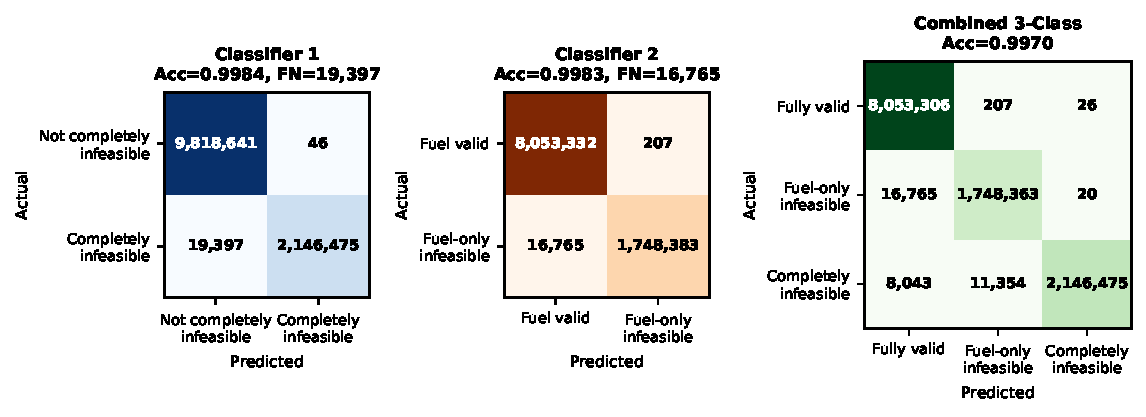
\includegraphics[width=\textwidth]{step7_classification_confusion.pdf}
\caption{Confusion matrices of the two classifiers and the combined three-class decision.}
\label{fig:confusion}
\end{figure*}

\subsection{Regression accuracy}\label{sec:regacc}
\autoref{tab:regression} reports the per-output accuracy of the regression stage on the primary screening-disjoint test subset. Each output was evaluated only on rows for which that target is defined by the simulator, independently of the predicted feasibility decisions. \autoref{fig:scatter} compares the surrogate predictions with the simulator values for all ten outputs using the corresponding target-valid rows. To provide a dimensionless comparison across outputs with different units, the relative MAE in \autoref{tab:regression} is expressed as a percentage of each output's standard deviation. Under this normalisation, the error remains below 1.5\% of the standard deviation for every output, with $R^2\geq0.9994$ throughout. Ship speed is over-predicted in 40.7\% of the positive-target cases, while the remaining nine outputs are over-predicted in 51.5--76.9\% of cases. Therefore, in the reported run every output errs preferentially on its specified safe side; the margin is small for motion sickness incidence (51.5\%). The same holds for seed 1, whereas seed 2 places nine of the ten outputs on their safe side, with ship speed over-predicted in 61.4\% of the positive-target cases (\autoref{tab:seeds}). \autoref{fig:residuals} presents the residual distributions, while \autoref{fig:seaheat} shows the range-normalised MAE across the evaluated sea-condition bands, i.e.\ the MAE within each significant-wave-height band (0--2, 2--5, 5--8, and 8--10~m, lower bound inclusive) expressed as a percentage of the output's range over the test rows on which it is defined.
\begin{table*}[ht]
\centering
\caption{Regression accuracy on the primary test subset.}
\label{tab:regression}
\footnotesize
\setlength{\tabcolsep}{7pt}
\begin{tabular}{
  l
  S[table-format=2.7]
  S[table-format=2.7]
  S[table-format=1.5]
  S[table-format=1.2]
  S[table-format=2.1]
}
\toprule
Output & {MAE} & {RMSE} & {$R^2$} & {Rel.\ MAE [\%]} & {Over-pred.\ [\%]} \\
\midrule
Ship speed [\unit{kn}]          & 0.01939   & 0.02800   & 0.99991 & 0.67 & 40.7 \\
Brake power [\unit{kW}]         & 47.87     & 62.87     & 0.99992 & 0.68 & 75.0 \\
Brake torque [\unit{kNm}]       & 3.289     & 4.280     & 0.99992 & 0.68 & 72.4 \\
Lateral acc.\ RMS [$g$]         & 0.0001634 & 0.0002276 & 0.99983 & 0.94 & 64.9 \\
Motion sickness [\%]            & 0.05683   & 0.09420   & 0.99990 & 0.61 & 51.5 \\
Rolling RMS [\unit{\degree}]    & 0.02236   & 0.03305   & 0.99965 & 1.26 & 71.1 \\
Slamming prob.\ [\%]            & 0.007542  & 0.01526   & 0.99982 & 0.67 & 76.9 \\
Green water prob.\ [\%]         & 0.03184   & 0.06111   & 0.99987 & 0.60 & 58.7 \\
Prop.\ emergence [\%]           & 0.09130   & 0.1572    & 0.99992 & 0.52 & 59.8 \\
Fuel consumption [\unit{kg/nm}] & 0.4273    & 1.043     & 0.99940 & 1.00 & 74.0 \\
\bottomrule
\end{tabular}
\end{table*}
\begin{table*}[ht]
\centering
\caption{Seed variability of the regressor (\checkmark{} = conservative side).}
\label{tab:seeds}
\footnotesize
\setlength{\tabcolsep}{6pt}
\begin{tabular}{
  l
  c
  S[table-format=1.5]
  c
  c
}
\toprule
Output & {$R^2$ Mean $\pm$ SD} & {Min.\ $R^2$} & {MAE Mean $\pm$ SD} & {Over-pred.\ [\%] (seeds 0/1/2)} \\
\midrule
Ship speed             & $0.99989 \pm 2.2 \times 10^{-5}$ & 0.99987 & $0.02120 \pm 0.0028$ & 40.7\,\checkmark{} / 41.9\,\checkmark{} / 61.4 \\
Brake power            & $0.99991 \pm 2.1 \times 10^{-5}$ & 0.99989 & $51.16 \pm 5.9$ & 75.0 / 66.3 / 64.2 (all \checkmark) \\
Brake torque           & $0.99990 \pm 2.2 \times 10^{-5}$ & 0.99988 & $3.688 \pm 0.42$ & 72.4 / 72.6 / 67.3 (all \checkmark) \\
Lateral acc.\ RMS      & $0.99980 \pm 6.3 \times 10^{-5}$ & 0.99972 & $0.0001797 \pm 3 \times 10^{-5}$ & 64.9 / 66.2 / 59.4 (all \checkmark) \\
MSI                    & $0.99980 \pm 8.1 \times 10^{-5}$ & 0.99975 & $0.08192 \pm 0.022$ & 51.5 / 81.7 / 66.3 (all \checkmark) \\
Roll RMS               & $0.99964 \pm 6.5 \times 10^{-5}$ & 0.99957 & $0.02323 \pm 0.0025$ & 71.1 / 67.8 / 68.3 (all \checkmark) \\
Slamming prob.         & $0.99976 \pm 9.9 \times 10^{-5}$ & 0.99964 & $0.008246 \pm 0.0022$ & 76.9 / 59.1 / 82.0 (all \checkmark) \\
Green water prob.      & $0.99983 \pm 7.3 \times 10^{-5}$ & 0.99975 & $0.03494 \pm 0.0053$ & 58.7 / 58.8 / 62.0 (all \checkmark) \\
Prop.\ emergence prob. & $0.99987 \pm 4.7 \times 10^{-5}$ & 0.99984 & $0.1232 \pm 0.028$ & 59.8 / 75.4 / 65.3 (all \checkmark) \\
Fuel consumption       & $0.99927 \pm 1.6 \times 10^{-4}$ & 0.99909 & $0.5180 \pm 0.089$ & 74.0 / 80.5 / 68.4 (all \checkmark) \\
\bottomrule
\end{tabular}
\end{table*}

\begin{figure*}[ht!]
\centering
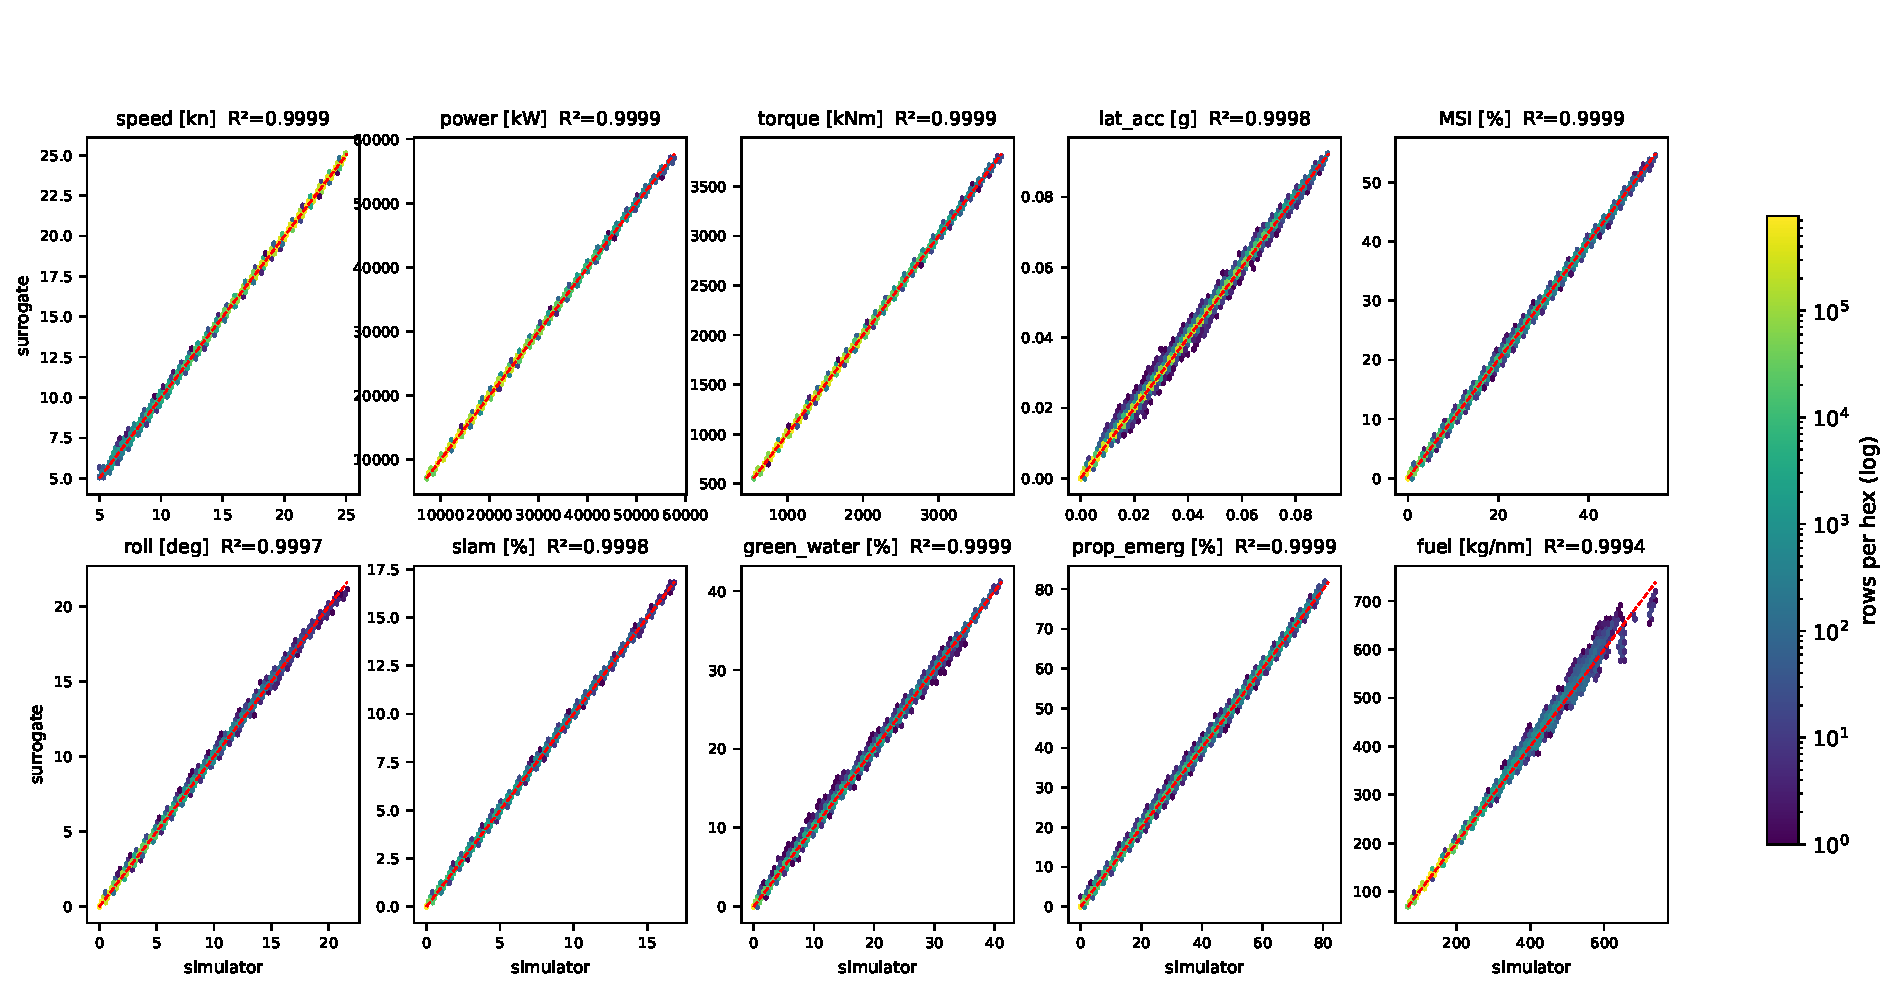
\includegraphics[width=1.0\textwidth]{fig_pred_vs_true.pdf}
\caption{Predicted against simulator values on the primary test subset (log-density).}
\label{fig:scatter}
\end{figure*}
\begin{figure*}[ht!]
\centering
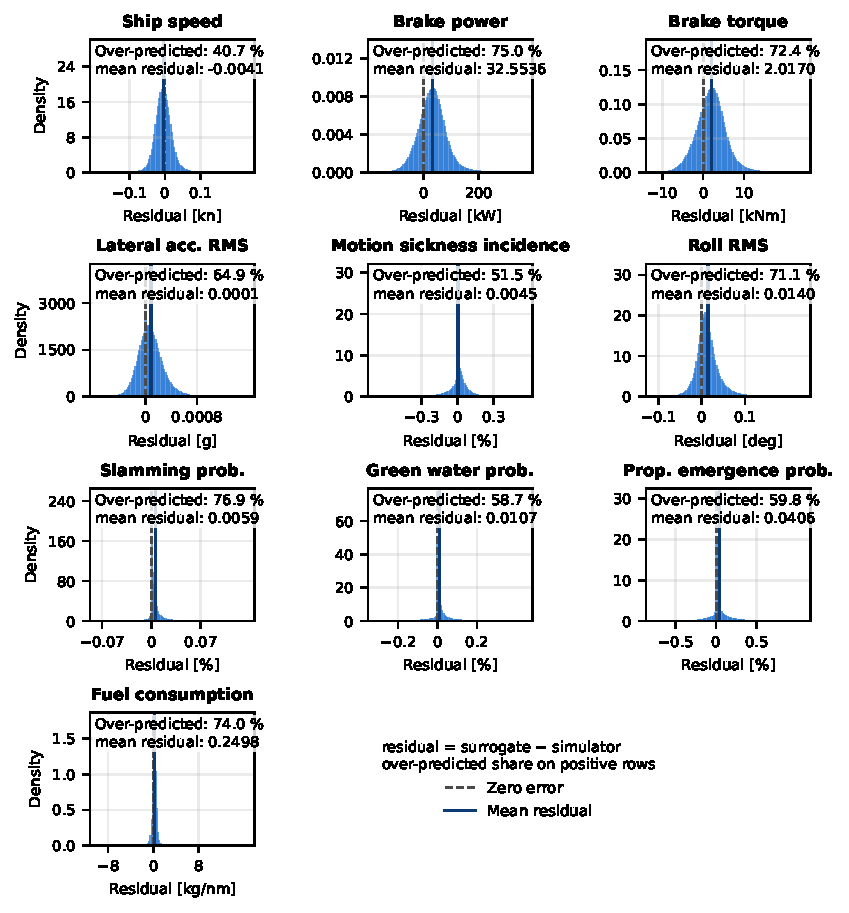
\includegraphics[width=0.75\textwidth]{step7_residual_distributions.pdf}
\caption{Residual distributions of the ten regression outputs.}
\label{fig:residuals}
\end{figure*}
\begin{figure*}[htpb]
\centering
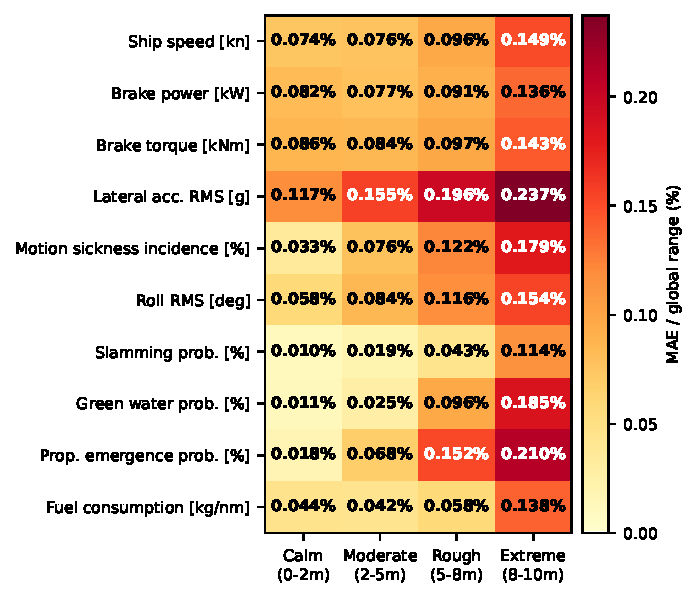
\includegraphics[width=\textwidth]{step7_error_heatmap_sea_conditions.pdf}
\caption{Range-normalised MAE by output and wave-height band.}
\label{fig:seaheat}
\end{figure*}

\subsection{Generalisation to unseen operating conditions}\label{sec:general}
\autoref{tab:general} summarises the structured holdout regimes of \autoref{sec:method}, in which the test conditions are excluded from training by construction rather than sampled at random, and \autoref{fig:r2heat} resolves the same regimes per output. In \autoref{tab:general}, the minimum $R^2$ is the worst result among the ten outputs, and the dangerous-pass rates are the percentages of completely infeasible and fuel-only-infeasible rows that the assembled surrogate passes as feasible; the fuel-only rate therefore refers to the cascade and can differ from the standalone $C_2$ rate shown in \autoref{fig:clffnr}. The loss of accuracy differs markedly between regimes. Holding out entire levels of wave height, wave direction, or wind speed leaves both the regression accuracy (minimum output $R^2 \geq 0.9985$) and the feasibility decision (accuracy $\geq 0.9911$) close to the random-split reference, so the surrogate transfers to unseen values of the environmental inputs; the exception is the wind-speed holdout, in which 2.39\% of completely infeasible conditions are passed as feasible, compared with 0.90\% on the random split. The draft holdout is harder: the design contains only three draft values, so removing one removes a third of the loading envelope, and \autoref{fig:r2heat} localises the loss of accuracy to the seakeeping outputs, with the minimum output $R^2$ dropping to 0.921 (slamming probability) while ship speed, brake power, and brake torque retain $R^2\geq0.9969$ and fuel consumption $R^2=0.989$; the recall of the standalone fuel-only classifier falls to 0.905. The block holdout, which removes a contiguous joint region of the envelope, retains a minimum $R^2$ of 0.992, and the corner regime, which tests genuine extrapolation outside the trained envelope, retains $R^2 \geq 0.980$ for all outputs but degrades the detection of completely infeasible conditions substantially: 11.2\% of completely infeasible corner rows are passed as feasible, against 0.9\% on the random split. The behaviour of both classifiers across all seven regimes is collected in \autoref{fig:clffnr}, which plots their test false-negative rates against the 1\% level implied by the validation recall floor: the rates remain below 2.5\% in all regimes except for the fuel classifier under the draft holdout (9.5\%) and the complete-infeasibility classifier under the block (4.1\%) and corner (11.2\%) regimes, so that, apart from the draft holdout, which also degrades the regression accuracy, the feasibility boundary rather than the regression surface is what limits transfer.
\begin{figure*}[ht!]
\centering
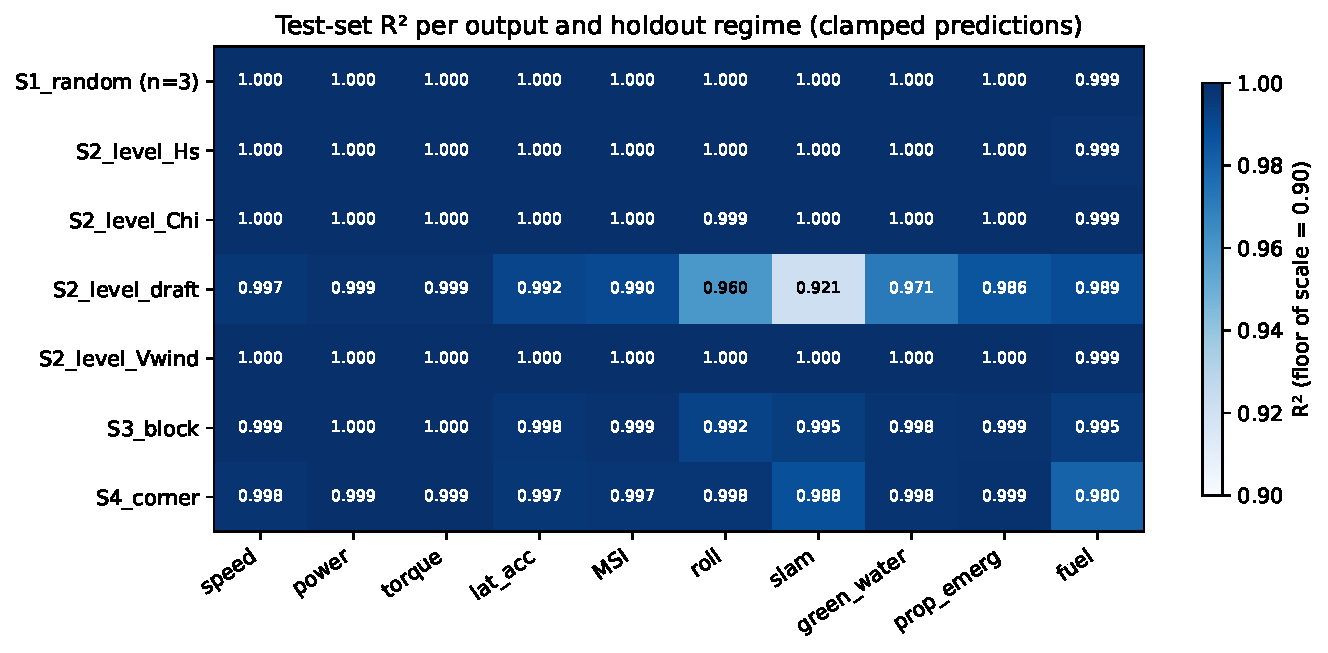
\includegraphics[width=0.65\textwidth]{fig_r2_heatmap.pdf}
\caption{Test-set $R^2$ per output and holdout regime.}
\label{fig:r2heat}
\end{figure*}

\begin{figure*}[ht!]
\centering
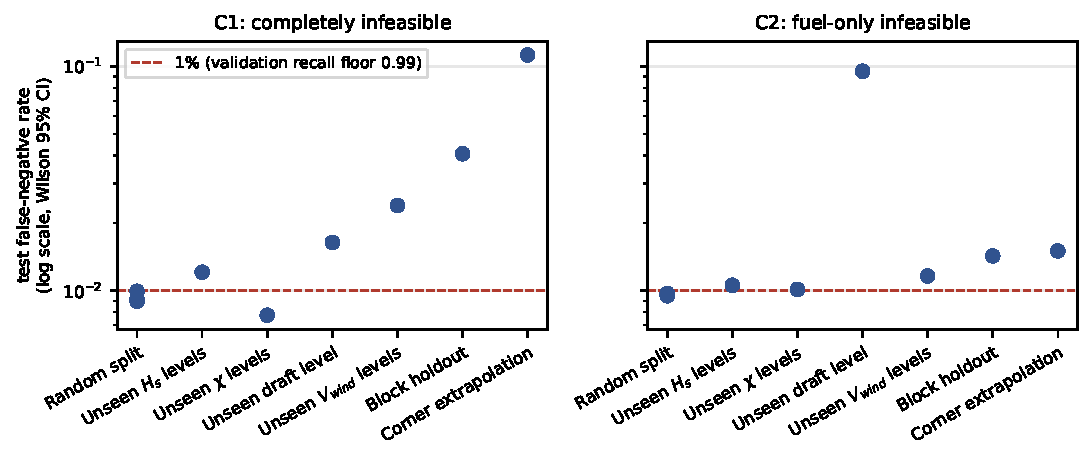
\includegraphics[width=\textwidth]{fig_clf_fnr.pdf}
\caption{Test false-negative rates of both classifiers across the holdout regimes.}
\label{fig:clffnr}
\end{figure*}
\begin{table*}[ht]
\centering
\caption{Generalisation across the holdout regimes.}
\label{tab:general}
\footnotesize
\setlength{\tabcolsep}{10pt}
\begin{tabular}{
  l
  S[table-format=8.0]
  S[table-format=1.4]
  S[table-format=1.4]
  S[table-format=2.2]
  S[table-format=1.2]
}
\toprule
 & {Test Rows} 
 & {3-Class} 
 & {Min.} 
 & \multicolumn{2}{c}{Dangerous Incorrect Pass [\%]} \\
\cmidrule(lr){5-6}
Regime & {(count)} & {Accuracy} & {$R^2$} & {Complete} & {Fuel-only} \\
\midrule
Random split                      & 11984559 & 0.9970 & 0.9994 &  0.90 & 0.95 \\
Unseen $H_s$ levels               &  8772594 & 0.9959 & 0.9985 &  1.21 & 1.05 \\
Unseen $\chi$ levels              &  9717344 & 0.9968 & 0.9993 &  0.77 & 1.01 \\
Unseen draft level                & 39935793 & 0.9768 & 0.9212 &  1.64 & 7.74 \\
Unseen $V_{\mathrm{wind}}$ levels & 39949087 & 0.9911 & 0.9990 &  2.39 & 1.16 \\
Block holdout                     & 11296734 & 0.9937 & 0.9924 &  4.07 & 1.42 \\
Corner extrapolation              & 34589019 & 0.9613 & 0.9804 & 11.22 & 1.46 \\
\bottomrule
\end{tabular}
\end{table*}
Complementing the holdout regimes, which reuse the precomputed factorial table, the simulator itself was re-run at input combinations in which all nine varying inputs simultaneously take values strictly between the training grid levels, providing validation against fresh simulator reference data that cannot be an artefact of the precomputed table. \autoref{tab:external-multidim} compares the surrogate with these new simulator results at 4{,}608 midpoint combinations (3{,}370 fully feasible) and 54{,}675 irregularly placed combinations (36{,}167 fully feasible). Accuracy, evaluated on the cases for which each output is defined (3{,}787 midpoint and 42{,}350 irregular cases for the nine non-fuel outputs, and the 3{,}370 and 36{,}167 fully feasible cases for fuel consumption), is preserved at both placements, with $R^2\geq0.9959$ for every output. Regression accuracy remains comparable across the two placement schemes, and neither placement is uniformly more difficult across the ten outputs. Both designs are full factorials of selected off-grid input values. In the midpoint design ($2\times2\times2\times3\times4\times3\times4\times2\times2$ combinations), every varying input takes values halfway between two adjacent training-grid levels, whereas the irregular design ($3\times3\times3\times3\times5\times3\times5\times3\times3$ combinations) uses off-grid values that are not midpoints, for example $\chi\in\{7.3^\circ,33.8^\circ,71.6^\circ,118.4^\circ,167.2^\circ\}$; no value of either design coincides with a training-grid level, and the complete value lists are provided in the code repository. The engineered error direction also largely transfers off-grid: all ten outputs err preferentially on their specified conservative side at the midpoint placements, whereas eight of ten do so at the irregular placements, where ship speed is over-predicted in 69.3\% and propeller-emergence probability in only 48.4\% of the positive-target cases (\autoref{tab:external-multidim}).

The fresh off-grid runs also probe the feasibility stage on newly generated infeasible cases. The completely-infeasible classifier keeps its in-distribution recall at the midpoints (0.991, false-negative rate 0.9\% with 95\% Wilson interval $[0.4, 1.7]\%$ over 821 infeasible cases), but at irregular placements its recall falls to 0.911 (false-negative rate 8.9\%, $[8.4, 9.4]\%$, 12{,}325 cases), mirroring the corner-regime finding that the feasibility boundary transfers less readily than the response surface. The fuel-only classifier shows the opposite pattern: recall 0.945 at irregular placements (5.5\%, $[5.0, 6.1]\%$) but only 0.791 at the midpoints (20.9\%, $[17.2, 25.0]\%$, over the small population of 417 fuel-only cases), showing that fuel-feasibility classification generalises less reliably to the midpoint placement. Off-grid use of the feasibility decision therefore requires either a lower decision threshold for the infeasible class, selected using representative off-grid validation data, or an explicit safety margin near the operating-envelope boundary.

The originally supplied interpolation scheme was evaluated on the same fresh off-grid points as an accuracy baseline, implemented as it operates in deployment: multilinear interpolation over the precomputed factorial table in the nine varying inputs (\autoref{tab:interpbaseline}). For the nine non-fuel outputs, all bracketing nodes are feasible for 70.2\% of the midpoint queries and 79.8\% of the irregular queries for which the simulator returns these outputs. For fuel consumption, the corresponding clean-cell proportions are 58.4\% and 75.2\%, because 41.6\% and 24.8\% of the respective queries with a valid fuel consumption have at least one fuel-infeasible bracketing node. On the matched clean-cell rows, which are restricted to simulator-feasible cases, the surrogate achieves, at full precision, higher $R^2$ in 17 of the 20 output--design combinations and is marginally lower in three, brake torque and fuel consumption at the midpoint placements and brake torque at the irregular placements, by at most $8\times10^{-4}$; the last of these and slamming probability at the irregular placements are equal at the displayed precision. The largest advantage of the surrogate occurs for slamming probability at the midpoint placements, where the interpolant obtains $R^2 = 0.9622$ compared with $R^2 = 0.9959$ for the surrogate. The remaining 20--30\% of queries, rising to 41.6\% for fuel consumption at the midpoint placements, lie in cells containing at least one infeasible grid node. In these cases, naive interpolation blends the $-1$ infeasibility encoding into the physical values and therefore does not preserve the feasibility boundary. These results show that the interpolation scheme is generally less accurate than the learned surrogate even within fully feasible cells and, more importantly, does not preserve the feasibility boundary when the interpolation cell contains infeasible grid nodes.

\begin{table*}[ht]
\centering
\caption{Off-grid validation against fresh simulator runs; regression metrics on the cases for which each output is defined (\checkmark{} = conservative side).}
\label{tab:external-multidim}
\footnotesize
\setlength{\tabcolsep}{6pt}

\begin{tabular}{
  l
  c
  S[table-format=1.5]
  S[table-format=2.1]
  c
  S[table-format=1.5]
  S[table-format=2.1]
}
\toprule
& \multicolumn{3}{c}{Midpoint Placement}
& \multicolumn{3}{c}{Irregular Placement} \\
\cmidrule(lr){2-4}
\cmidrule(lr){5-7}

Output
& {MAE}
& {$R^2$}
& {Over-pred.\ [\%]}
& {MAE}
& {$R^2$}
& {Over-pred.\ [\%]} \\
\midrule

Ship speed [\unit{kn}]
& 0.0396
& 0.99956
& \safe{40.0}
& 0.0497
& 0.99944
& 69.3 \\

Brake power [\unit{kW}]
& 160.5
& 0.99901
& \safe{92.8}
& 127.6
& 0.99945
& \safe{68.8} \\

Brake torque [\unit{kNm}]
& 16.72
& 0.99803
& \safe{97.8}
& 11.13
& 0.99919
& \safe{82.4} \\

Lateral acc.\ RMS [$g$]
& 0.000310
& 0.99931
& \safe{66.6}
& 0.000279
& 0.99929
& \safe{56.6} \\

Motion sickness [\%]
& 0.0980
& 0.99940
& \safe{65.4}
& 0.0916
& 0.99961
& \safe{51.2} \\

Rolling RMS [\unit{\degree}]
& 0.0562
& 0.99758
& \safe{65.4}
& 0.0580
& 0.99671
& \safe{75.3} \\

Slamming prob.\ [\%]
& 0.0106
& 0.99592
& \safe{59.1}
& 0.0134
& 0.99755
& \safe{78.1} \\

Green water prob.\ [\%]
& 0.0472
& 0.99888
& \safe{58.4}
& 0.0606
& 0.99929
& \safe{59.3} \\

Prop.\ emergence [\%]
& 0.1221
& 0.99976
& \safe{55.3}
& 0.1651
& 0.99963
& 48.4 \\

Fuel consumption [\unit{kg/nm}]
& 1.190
& 0.99766
& \safe{90.2}
& 0.8925
& 0.99913
& \safe{60.1} \\

\bottomrule
\end{tabular}
\end{table*}
\begin{table*}[ht]
\centering
\caption{Multilinear interpolation baseline against the surrogate on fresh off-grid runs: $R^2$ on clean cells (all bracketing grid nodes feasible) and share of contaminated queries (at least one infeasible bracketing node).}
\label{tab:interpbaseline}
\footnotesize
\setlength{\tabcolsep}{5pt}
\begin{tabular}{
  l
  S[table-format=1.4]
  S[table-format=1.4]
  S[table-format=1.4]
  S[table-format=1.4]
  S[table-format=2.1]
  S[table-format=2.1]
}
\toprule
 & \multicolumn{2}{c}{Midpoint, Clean $R^2$} 
 & \multicolumn{2}{c}{Irregular, Clean $R^2$} 
 & \multicolumn{2}{c}{Contaminated [\%]} \\
\cmidrule(lr){2-3} \cmidrule(lr){4-5} \cmidrule(lr){6-7}
Output & {Interp.} & {Surrogate} & {Interp.} & {Surrogate} & {Midpoint} & {Irregular} \\
\midrule
Ship speed             & 0.9979 & 0.9994 & 0.9977 & 0.9993 & 29.8 & 20.2 \\
Brake power            & 0.9983 & 0.9989 & 0.9991 & 0.9994 & 29.8 & 20.2 \\
Brake torque           & 0.9985 & 0.9978 & 0.9991 & 0.9991 & 29.8 & 20.2 \\
Lateral acc.\ RMS      & 0.9983 & 0.9994 & 0.9976 & 0.9994 & 29.8 & 20.2 \\
Motion sickness        & 0.9956 & 0.9995 & 0.9965 & 0.9996 & 29.8 & 20.2 \\
Rolling RMS            & 0.9935 & 0.9972 & 0.9944 & 0.9961 & 29.8 & 20.2 \\
Slamming prob.         & 0.9622 & 0.9959 & 0.9975 & 0.9975 & 29.8 & 20.2 \\
Green water prob.      & 0.9901 & 0.9988 & 0.9990 & 0.9993 & 29.8 & 20.2 \\
Prop.\ emergence prob. & 0.9975 & 0.9998 & 0.9987 & 0.9997 & 29.8 & 20.2 \\
\addlinespace
Fuel consumption       & 0.9970 & 0.9966 & 0.9954 & 0.9990 & 41.6 & 24.8 \\
\bottomrule
\end{tabular}
\end{table*}

\subsection{Computational performance}\label{sec:speed}
The simulator and surrogate were evaluated on the same workstation described in \autoref{sec:env}, and the workload-matched results are reported in \autoref{tab:timing}. The reported ratios represent system-level wall-clock comparisons because the simulator executes on the CPU, whereas the surrogate performs inference on the GPU. The simulator single-point time of 8.939~s is the median of ten separate process invocations, while the surrogate single-point latency of 2.646~ms is the mean per call over 864 sequential evaluations, corresponding to a point-to-point speed-up of approximately $3{,}378$. On the identical 864-point timing grid, the complete surrogate evaluates the batch in 2.744~ms, while the simulator's batch mode requires 14.338~s (median of three invocations), corresponding to a batch-to-batch speed-up of approximately $5{,}226$. Both ratios are computed from the recorded times, which carry more digits than those shown in \autoref{tab:timing}. Because every simulator invocation incurs a per-invocation cost in addition to the evaluation of its operating points, the single-point ratio characterises isolated queries, whereas the 864-point comparison, in which this cost is shared by all points of one invocation (approximately 16.6~ms per point), is more representative of repeated evaluation. \autoref{tab:speed} reports the separate large-batch throughput experiment. At a batch size of 65{,}536, the complete pipeline reaches approximately $4.03\times10^6$ predictions per second, equivalent to an amortised cost of approximately 0.25~\textmu s per point. This value represents large-batch throughput and should not be interpreted as single-query latency.
\begin{table*}[ht]
\centering
\caption{Workload-matched wall-clock comparison on the same workstation.}
\label{tab:timing}
\begin{tabular}{lrrr}
\hline
Matched workload & Simulator wall time & Surrogate wall time & Speed-up \\
\hline
Single-point evaluation & 8.939\,s & 2.646\,ms & $\times3{,}378$ \\
Identical 864-point batch & 14.338\,s & 2.744\,ms & $\times5{,}226$ \\
\hline
\end{tabular}
\end{table*}
\begin{table}[ht]
\centering
\caption{GPU inference throughput for the regressor and the complete pipeline.}
\label{tab:speed}
\footnotesize
\setlength{\tabcolsep}{12pt}
\begin{tabular}{
  S[table-format=6.0]
  S[table-format=8.0]
  S[table-format=7.0]
}
\toprule
{Batch Size} & {Regressor [pred/s]} & {Full Pipeline [pred/s]} \\
\midrule
   512 &  667952 & 198065 \\
  4096 & 5337465 & 1590160 \\
 16384 & 10640340 & 3584977 \\
 65536 & 11479858 & 4032683 \\
262144 & 12402518 & 4079985 \\
\bottomrule
\end{tabular}
\end{table}
\section{Discussion}\label{sec:discussion}
The results in \autoref{sec:results} show that the two-stage surrogate reproduces the S175 model closely across all ten outputs while preserving the structure of its feasible operating envelope. On the held-out test set the mean absolute error remains below 1.5\% of the standard deviation of every output, with $R^2 \geq 0.9994$ throughout (\autoref{tab:regression}, \autoref{fig:scatter}), and the combined feasibility decision reproduces the infeasibility structure of the simulator for 99.70\% of the test rows (\autoref{tab:classifiers}, \autoref{fig:confusion}). This addresses the central limitation identified in \autoref{sec:related}: a single continuous regression surrogate would return numerical outputs also for conditions in which the simulator returns none, whereas the two-stage design first decides feasibility and only then predicts output values, so that the surrogate is built to decline to answer where the physics-based model does, and does so with high fidelity in distribution. Because the decision thresholds are selected on validation for a recall of at least 0.99 of the infeasible class, the rate of dangerous false negatives observed on the random test split is about 1\%, matching the validation target; this is an empirical result under the test distribution, not a guarantee: among the structured holdout regimes it rises to 9.5\% for the standalone fuel-only classifier under the draft holdout and to 11.2\% for the complete-infeasibility classifier under corner extrapolation, and at off-grid inputs the fuel-only classifier reaches a false-negative rate of 20.9\% at midpoint placements (\autoref{sec:results}), the largest feasibility failure measured in this study. The full threshold sweep is retained with the trained models, so a deployment requiring a stricter operating point on a given distribution can re-select the threshold without retraining.

The per-output asymmetric loss makes the direction of the prediction error, rather than only its magnitude, usable for conservative route evaluation. The five-arm ablation in \autoref{tab:lossablation} separates the effects of batch-normalisation placement, masked training, and output-specific weighting. The original configuration places three of ten outputs on their safe side, the corrected but unmasked configuration places two, the uniform masked configuration places one, and the symmetric masked configuration places six. Only the selected per-output masked configuration places all ten outputs on their safe side. The resulting over-prediction rates range from 51.5\% to 76.9\% for the nine outputs biased toward over-prediction, while ship speed is over-predicted in 40.7\% of cases. Across the three training seeds, two runs place all ten outputs on their safe side and one places nine (\autoref{tab:seeds}). This directional bias is distributional rather than a per-prediction guarantee; individual predictions can still err on the unsafe side, and applications requiring hard one-sided bounds should combine the surrogate with calibrated uncertainty estimates or explicit safety margins. The bias nevertheless largely persists off-grid, where all ten outputs remain on their safe side at midpoint placements and eight of ten do so at irregular placements. The loss-weight selection is conditional on the finite prespecified grid. Because the selected value $\alpha_{\mathrm{other}}=0.33$ lies at the lower boundary of that grid, the experiment establishes the only eligible pair among the evaluated configurations but not the optimal continuous value near or beyond the tested boundary.

The generalisation experiments in \autoref{tab:general} distinguish interpolation within the densely sampled factorial grid from transfer to systematically withheld operating conditions. Withholding complete levels of the environmental inputs produces limited regression degradation, with a minimum output $R^2\geq0.9985$, whereas the block holdout produces a more noticeable reduction, with $R^2\geq0.992$. The draft and corner regimes identify the principal limitations. Withholding one of only three draft levels reduces the minimum $R^2$ to 0.921 and the recall of the standalone fuel-only classifier to 0.905, indicating that the loading conditions are too sparsely sampled to support omission of an entire draft level. Under corner extrapolation, regression accuracy remains above $R^2=0.980$, but 11.2\% of completely infeasible conditions are incorrectly passed as feasible, compared with 0.9\% on the random split. The fresh off-grid evaluations in \autoref{tab:external-multidim} confirm that the regression stage remains accurate at intermediate input positions, with $R^2\geq0.9959$ for every output, while the feasibility results show greater sensitivity to leaving the training grid. The interpolation comparison in \autoref{tab:interpbaseline} provides additional context: when an interpolation cell contains infeasible nodes, direct multilinear interpolation blends the infeasibility encoding with physical values and therefore cannot preserve the feasibility boundary. Within clean cells, the surrogate achieves a higher $R^2$ in 17 of the 20 output--placement comparisons. The agreement with fresh simulator runs also confirms that the reported accuracy is not an artefact of the precomputed factorial table, and the comparison across regimes shows that the feasibility boundary is markedly harder to extrapolate than the smooth response surfaces.
The computational comparison in \autoref{tab:timing} demonstrates that the acceleration remains substantial under workload-matched conditions. The surrogate is approximately $3{,}378$ times faster for single-point evaluation, requiring 2.646~ms instead of 8.939~s, and approximately $5{,}226$ times faster when both systems evaluate the identical 864-point batch. The large-batch cost of approximately 0.25~\textmu s per point is reported separately because it represents amortised GPU throughput rather than single-query latency. At the measured full-pipeline throughput of approximately $4.03\times10^6$ evaluations per second for a batch size of 65{,}536, processing 126.2 million surrogate inputs would require approximately 31 seconds, excluding data-transfer and routing-optimiser overheads. A corresponding full-dataset simulator time is not inferred because the measured simulator cost per point varies across batch sizes and operating-condition compositions. This acceleration provides the computational capacity required for evaluation-intensive operating-envelope analysis and weather-routing optimisation, although the end-to-end benefit within a complete routing system remains to be measured.



\section{Conclusion}\label{sec:conclusion}
This work developed a data-driven machine-learning surrogate for the physics-based S175 WeatherRouting performance simulator while explicitly modelling both its numerical outputs and feasibility structure. A full-factorial database of 126{,}153{,}720 simulator evaluations over nine varying inputs was generated. The resulting two-stage architecture first identifies fully valid, fuel-only-infeasible, and completely infeasible operating conditions and then uses a multi-output multi-layer perceptron to predict the ten performance and seakeeping outputs for which valid targets exist. The regressor is trained using a masked, per-output asymmetric loss that directs its residuals preferentially toward the conservative side of each output.

On the primary screening-disjoint test subset, the surrogate attains $R^2\geq0.9994$ for all ten outputs, while the combined feasibility decision achieves an accuracy of 99.70\%, a balanced accuracy of 0.9938, and a macro-averaged F1 score of 0.9953. The structured-holdout and fresh off-grid evaluations show that the regression stage remains highly accurate for unseen environmental levels and intermediate off-grid inputs. They also identify the principal validity limits of the feasibility stage, particularly for the unseen-draft regime, corner extrapolation, and some off-grid placements. Under workload-matched comparisons, the surrogate is approximately $3{,}378$ times faster than the simulator for single-point evaluation and $5{,}226$ times faster for an identical 864-point batch. Its large-batch cost falls to approximately 0.25~\textmu s per point, although this value represents amortised throughput rather than single-query latency.

The principal limitations are that the surrogate measures fidelity to the simulator rather than physical-vessel accuracy, covers a finite set of loading and environmental conditions, and requires a substantial initial data-generation effort. Future work will therefore extend the database to broader operating and loading conditions, investigate data-efficient sampling and calibrated uncertainty estimates, validate the modelling chain against experimental or full-scale observations when suitable data become available, and integrate the surrogate into a complete weather-routing optimisation framework.

\section*{Code availability}
The complete implementation is publicly available in the \href{https://github.com/MOHAMMED-ABDALSALAM-PG/S175-ML-surrogate}{S175-ML-surrogate GitHub repository}. The repository contains the training, evaluation, and figure-generation code, the experiment configurations, the split definitions with SHA-256 checksums, the trained model checkpoints for every reported run together with their full provenance records (configuration, seed, data and split hashes, and library versions), and the scripts that regenerate every table and figure in this paper from the recorded results. The dataset and the S175 WeatherRouting simulator are not redistributed; the dataset is available from the corresponding author upon reasonable request.

\section*{Data availability}
The dataset generated and analysed during the current study (126{,}153{,}720 evaluations of the S175 WeatherRouting simulator, 15.9~GB) is not publicly deposited owing to its size, but is available on reasonable request from the corresponding author, Prof. Joanna Sz{\l}apczy{\'n}ska (joanna.szlapczynska@pg.edu.pl). The trained model checkpoints, the split definitions with SHA-256 checksums, and all evaluation tables underlying the figures are publicly available in the code repository listed under Code availability.
\section*{CRediT authorship contribution statement}

\textbf{Mohammed Abdalsalam:} Methodology, Software, Formal analysis, Investigation, Visualization,
Writing -- original draft, Writing -- review \& editing.\\
\textbf{Aleksander Kniat:} Software, Resources, Data curation, Validation,
Writing -- review \& editing.\\
\textbf{Przemys{\l}aw Krata:} Software, Validation, Writing -- original draft,
Writing -- review \& editing.\\
\textbf{Joanna Sz{\l}apczy{\'n}ska:}  Conceptualization, Methodology, Formal analysis, Validation, Writing -- review \& editing, Supervision, Project Administration.


\section*{Acknowledgements}
The authors gratefully acknowledge PhD Eng. Roberto Vettor for developing the theoretical general ship model underlying the S175 WeatherRouting performance simulator employed in this study. This work was originally carried out within the international MarTERA-1 ROUTING project (2018–2022), under the supervision of Prof. Carlos Guedes Soares at Instituto Superior Técnico, Lisbon, Portugal. The authors sincerely appreciate their foundational contributions to the formulation and development of the ship-performance model.
\section*{Declaration of competing interest}
The authors declare no competing interests.
\bibliographystyle{elsarticle-num}
\bibliography{sample}

\end{document}
